\documentclass[a4paper,fleqn,12pt]{article}

\usepackage[utf8]{inputenc}
\usepackage[bulgarian]{babel}
\usepackage{amsmath}
\usepackage{amssymb}
\usepackage{booktabs}
\usepackage{fancyhdr}
\usepackage{amsthm}
\usepackage{graphicx}

\theoremstyle{definition}
\newtheorem{theorem}{Tеорема}[subsection]
\newtheorem{lemma}[theorem]{Лема}

\newtheorem{definition}{Дефиниция}[subsection]

\newtheorem{example}{Пример}[subsection]

\newtheorem{task}{Задача}[subsection]



\title{Математически анализ 2}
\author{Exonaut}

\pagestyle{fancy}
\fancyhf{}
\lhead{\rightmark}
\rhead{\thepage}
\cfoot{}
\renewcommand{\headrulewidth}{0pt}


\begin{document}

\pagenumbering{gobble}
\maketitle

\newpage
\pagenumbering{arabic}

\tableofcontents
\newpage

\section{Лекция 1: Пространството $\mathbb{R}^m$}

\subsection{Няколко важни неравенства}
Нека $a_k $ и $b_k (k = 1, 2, ..., m) $ са реални числа и $m \in \mathbb{N}$
\begin{theorem}[Неравенство на Коши-Шварц]
В сила е следното неравенство: \\
$$\left( \sum_{k=1}^{m}a_kb_k \right ) ^ 2   \leq  \left( \sum_{k=1}^{m}a_k \right)  \left( \sum_{k=1}^{m}b_k  \right) $$
\end{theorem}
Равенство се достига само когато $a_k$ и $b_k$ са пропорционални:\\
 ($\exists \lambda_0: b_k =\lambda_0 a_k  $)\\
Равенството може да се запише: 
$$\displaystyle\left\lvert \sum_{k=1}^{m}a_kb_k \right \rvert \leq \sqrt{\left( \sum_{k=1}^{m}a_k \right)}  \sqrt{ \left( \sum_{k=1}^{m}b_k  \right)} $$

\begin{theorem}[Неравенство на Минковски]
В сила е следното неравенство: \\
$$\sqrt{ \sum_{k=1}^{m} (a_k + b_k)^2}   \leq \sqrt{ \sum_{k=1}^{m}a_k^2 } + \sqrt{ \sum_{k=1}^{m}b_k^2 }$$
\end{theorem}
Равенство се достига само когато $a_k$ и $b_k$ са пропорционални.
Общ случай на неравенството на Минковски:
$$\left ( \sum_{k=1}^{m} \vert a_k + b_k\vert ^p \right)^\frac{1}{p}   \leq\left ( \sum_{k=1}^{m}\vert a_k\vert ^p\right)^\frac{1}{p} + \left ( \sum_{k=1}^{m} \vert b_k\vert ^p \right)^\frac{1}{p}   ( p\geq 1)$$

\begin{theorem}
В сила е следното неравенство: \\
$$ \vert a_k + b_k\vert   \leq \sqrt{ \sum_{k=1}^{m} (a_k + b_k)^2} \leq   \sum_{k=1}^{m}\vert a_k - b_k\vert  $$
\end{theorem}

\subsection{Видове крайно мерни пространства}

\subsubsection{Линейно(Векторно) пространство}
	\begin{definition}
Нека L е линейно(векторно) пространство над полето $R$. В него има въведени две операции: събиране и умножение на вектор с число.
		\begin{enumerate}
 			\item $x,y \in L \implies z = x+ y \in L $
			\item $x \in L, \lambda \in \mathbb{R} \implies z = \lambda x \in L$
		\end{enumerate}
\end{definition}

\subsubsection{Евклидово пространство}
\begin{definition}
Крайномерното пространство L се нарича евклидово, ако в него е въведено скаларно произведение, т.е за всеки два елемента $x,y \in L$ може да се съпостави реално число $(x,y)$, удовлетворяващо свойствата за линейност, симетричност и положителна определеност.
	\begin{enumerate}
 		\item $x,y,z \in L ,\lambda \in \mathbb{R} \implies (x+y,z) = (x,z) + (y,z); (\lambda x,y) = \lambda(x,y)$
		\item $x,y \in L \implies (x,y) = (y,x)$
		\item $x \in L, x\neq 0 \implies (x,x) > 0 $
	\end{enumerate}
\end{definition}

\subsubsection{Метрично пространство}
\begin{definition}
Крайномерното пространство L се нарича метрично, ако в него е въведено разстояние (метрика) $\rho$, т.е за два елемента $x,y \in L$ може да се съпостави неотрицателно число  $\rho \geq 0 $  със следните свойства
	\begin{enumerate}
 		\item $\rho(x,x) = 0 ; \rho(x,y) > 0 , x\neq y $
		\item $\rho(x,y) = \rho(y,x)$
		\item $\rho(x,z) \leq \rho(x,y) + \rho(y,z). \forall x,y,z \in L$
	\end{enumerate}
Метрично пространство L с метрика $\rho$ се означава $(L,\rho)$
\end{definition}

\subsubsection{Нормирано пространство}
\begin{definition}
Пространството се нарича нормирано, ако в него е въведена норма $\Vert. \Vert$, т.е $\Vert.\Vert: L \to \mathbb{R}_0^+$ със свойства 
	\begin{enumerate}
 		\item $x = 0  \implies \Vert x \Vert = 0, x \neq 0  \implies \Vert x\Vert > 0$
		\item $x \in L, \lambda \in \mathbb{R} \implies \Vert \lambda x \Vert = \vert \lambda\vert   \Vert x \Vert$
		\item $x,y \in L \implies \Vert x+y\Vert \leq \vert x\vert  + \vert y\vert $
	\end{enumerate}
\end{definition}
\begin{theorem}
Ако L е нормирано пространство с дадена норма $\Vert . \Vert$, то L е метрично пространство, т.е равенството $\rho(x,y) = \Vert x - y \Vert$ дефинира  разстоянието в L
\end{theorem}

\subsection{Пространството $\mathbb{R}^m$ - дефиниция и основни свойства}

\begin{definition}
Множеството от наредени m-торки $a = (a_1, a_2, ... , a_m)$ от реални числа. Числата $a_1, a_2, ... , a_m$ се наричат съответно първа, втора, ..., m-та кордината на а.\\
\\
 Ако имаме $a = (a_1, a_2, ... , a_m), b = (b_1, b_2, ... , b_m), ; \lambda \in \mathbb{R} $ то
	\begin{enumerate}
		\item $a+b =(a_1, a_2, ... , a_m) +  (b_1, b_2, ... , b_m) = (a_1 + b_1, a_2+b_2, ... , a_m + b_m) \in \mathbb{R}^m$
		\item $ \lambda a =(\lambda a_1,\lambda a_2, ... , \lambda a_m) \in \mathbb{R}^m $\\
	\end{enumerate}
\end{definition}

\subsubsection{Скаларно произведение}
Скаларно произведение се дефинира : $$ (a,b) = \left( \sum_{k=1}^{m}a_kb_k \right )$$\\
С така въведено скаларно произведение пространството $R^m$ се превръща в евклидово.

\subsubsection{Норма и метрика}
С равенството:
$$\Vert a\Vert := \sqrt{ \sum_{k=1}^{m}(a_k)^2  }$$ \\
се въвежда норма в $\mathbb{R}^m$.
\\
 Нормата генерира метрика в $\mathbb{R}^m$ с формула: 
$$\rho(a,b) := \Vert a-b\Vert = \sqrt{ \sum_{k=1}^{m} (a_k - b_k)^2} $$

\subsubsection{Скаларен квадрат}
Скаларен квадрат: $a^2 = (a,a) = \sum _{k=1}^{m}a_k^2$

\subsubsection{Неравенство на Коши-Шварц, чрез скаларен квадрат}
Коши-Шварц чрез скаларен квадрат: $(a,b)^2 \leq a^2b^2$ и $\vert (a,b)\vert \leq \Vert a \Vert \Vert b \Vert$

\subsubsection{Неравенство на Минковски, чрез скаларен квадрат}
Неравенство на Минковски чрез скаларен квадрат: $\Vert a+b \Vert\leq \Vert a \Vert + \Vert b \Vert$

\subsection{Точки и множества в $\mathbb{R}^m$}

\subsubsection{Паралелепипед}

\begin{definition}
Множеството\\
$$\Pi (a; \delta_1, \delta_2, ... ,\delta_m) = \{ x \in \mathbb{R}^m: -\delta_k < x_k -a_k < \delta_k   \}$$
се нарича отворен паралелепипед в $\mathbb{R}^m$ с център точката а.\\
\\
Множеството\\
$$\widetilde\Pi (a; \delta_1, \delta_2, ... ,\delta_m) = \{ x \in\mathbb{R}^m: -\delta_k \leq x_k -a_k \leq \delta_k   \}$$
се нарича затворен паралелепипед в $R^m$ с център точката а.\\
\\
Ако $\delta_1 = \delta_2 = ... = \delta_m = \delta$, получените множества $\Pi (a; \delta)$ и $\widetilde\Pi (a; \delta)$ се  наричат съответно отворен и затворен куб в $\mathbb{R}^m$ с център а.
 \end{definition}

\subsubsection{Сфера и кълбо}

\begin{definition}
Нека числото r > 0. Множеството \\
$$B(a;r) = \{ x \vert  x \in \mathbb{R}^m, \rho(x,a) <r \} = \{ x\vert  x \in \mathbb{R}^m, \Vert x-a \Vert < r \}$$\\
се нарича отворено кълбо в $\mathbb{R}^m$ с център a и радиус r, множеството \\
$$\widetilde B(a;r) = \{ x \vert  x \in \mathbb{R}^m, \rho(x,a) \leq r \} = \{ x\vert  x \in \mathbb{R}^m, \Vert x-a \Vert \leq r \}$$\\
се нарича затворено кълбо в $\mathbb{R}^m$ с център a и радиус r, а множеството \\
$$S(a;r) = \{ x \vert  x \in \mathbb{R}^m, \rho(x,a) = r \} = \{ x\vert  x \in \mathbb{R}^m, \Vert x-a \Vert = r \}$$\\
се нарича сфера в $\mathbb{R}^m$ с център a и радиус r, а множеството \\
\end{definition}

\begin{definition}
Точката а се нарича
\begin{itemize}
	\item вътрешна за множеството А, ако съществува отворено кълбо $B(a,\varepsilon): B(a,\varepsilon) \subset A$
	\item външна за А, ако съществува $B(a,\varepsilon): B(a,\varepsilon) \subset \mathbb{R}^m \setminus  A$
	\item контурна за А, ако за всяко $\varepsilon > 0: B(a,\varepsilon) \cap A \neq \varnothing $ и \\ $ B(a,\varepsilon) \cap (\mathbb{R}^m \setminus  A) \neq \varnothing$
	\item изолирана ако съществува $\varepsilon > 0: B(a,\varepsilon) \cap A = \{ a \}$
\end{itemize}
	
\end{definition}

\begin{definition}
Множеството $A \subset \mathbb{R}^m $ се нарича 

\begin{itemize}
	\item отворено, ако всяка негова точка е вътрешна 
	\item затворено, ако неговото допълнение  $\mathbb{R}^m \setminus A$ е отворено
\end{itemize}

\end{definition}

\begin{definition}
Околност на дадена точка $a \in \mathbb{R}^m $ се нарича всяко отворено множество, което я съдържа. Означава се с $U_a$.
\end{definition}

\begin{definition}
Точка а се нарича точка на сгъстяване на множеството $A \subset \mathbb{R}^m $, ако всяка нейна околност $U_a$ съдържа поне една точка на А, различна от а, т.е $U_a \cap (A\setminus \{ a \} \neq \varnothing $
\end{definition}

\begin{definition}
Величината \\
$$d = d(A) = \sup_{a',a'' \in A} \rho(a';a'')$$\\
се нарича диаметър на множеството  $A \subset \mathbb{R}^m $.
\end{definition}

\begin{definition}
Множеството  $A \subset \mathbb{R}^m $ се нарича ограничено, ако съшествува кълбо(с краен радиус), което го съдържа.
\end{definition}

\begin{definition}
Множеството  $A \subset \mathbb{R}^m $ се нарича компактно, ако А е затворено и ограничено.
\end{definition}

\begin{definition}
Множеството   $x = (x_1, x_2, ... , x_m) \in \mathbb{R}^m $, чийто кординати са непрекъснати функции $x_k = x_k(t) (k = 1, 2, ..., m)$, дефинирани върху даден интервал [a,b] се нарича непрекъсната крива в $R^m$. t се нарича параметър на кривата.\\
Точките $x(a) = (x_1(a), x_2(a), ... , x_m(a))$ и $x(b) = (x_1(b), x_2(b), ... , x_m(b))$ се наричат начало и край на дадената крива. Ако $x(a) = x(b)$ кривата е затворена
\end{definition}

\begin{definition}
Нека $x^0 = (x_1^0, x_2^0, ... , x_m^0) \in \mathbb{R}^m$ и $\alpha_1, \alpha_2, ... , \alpha_m$ са фиксирани числа за които $\sum_{k=1}^{m}\alpha_k > 0$. Множеството от точки $x = (x_1, x_2, ... , x_m)$ чиито кординати се представят във вида \\
$$x_k = x_k^0 + \alpha_kt, k = 1, 2, ..., m , -\infty < t <\infty $$\\
се нарича права линия в пространството $R^m$, минаваща през точка $x^0$ по направление $(\alpha_1, \alpha_2, ... , \alpha_m).$
\end{definition}

\begin{definition}
Множеството  $A \subset \mathbb{R}^m $ се нарича свързано,  ако за всеки две негови точки съществува непрекъсната крива $\gamma$, която ги свързва и $\gamma \subset A$.
\end{definition}

\begin{definition}
Множеството  $A \subset \mathbb{R}^m $ се нарича област, ако е отворено и свързано. Ако е и затворено, то се нарича затворена област. 
\end{definition}

\begin{definition}
Област, всеки две точки на която могат да се съединят с отсечка, изцяло лежаща в нея, се нарича изпъкнала област. 
\end{definition}

\begin{definition}
Областа $A \subset \mathbb{R}^m $ се нарича звездообразна област, отностно точката $x^0 \in A$, ако за вскяка точка $x \in A$ отсечката $[x^0,x]$ лежи изцяло в А. 
\end{definition}

\subsection{Редици от точки в $\mathbb{R}^m$}

\begin{definition}
Редицата $\{ x^{(n)} \}_{n = 1} ^ \infty = \{x_1 ^{(n)}, x_2 ^{(n)}, ... , x_m^{(n)}\} $ се нарича редица от точки в $\mathbb{R}^m$, а редицата $\{ x_k ^{(n)}\}_{n=1} ^ \infty ( k = 1 \div m) $ - к-та кординатна редица. За по кратко редицата $\{ x^{(n)} \}_{n = 1} ^ \infty$ се означава $\{ x^{(n)} \}$
\end{definition}

\begin{definition}
Редицата $\{ y^{(l)} \}_{l = 1} ^ \infty$ се нарича поредица на редицата $\{ x^{(n)} \}$ и се означава:\\
$\{ x^{(n_l)} \}, l = 1, 2, ..., $ или $\{ x^{(n_l)} \}_{l = 1} ^ \infty$\\
ако за всяко l съществува такова $n_l$, че $y^{(l)} = x^{(n_l)}$, при това, ако $l' < l'' $, то $n_{l'}<n_{l''}$.
\end{definition}

\begin{definition}
Редицата $\{ x^{(n)} \}$ се нарича сходяща към точка $a \in \mathbb{R}^m$ (граница на редицата), ако за всяко $\varepsilon > 0$ съществува такова $N_0 > 0$, че за всяко $n > N_0$ е изпълено неравенството $\rho(x^{(n)};a) = \Vert x^{(n)} - a \Vert < \varepsilon$. Ако редицата няма граница, се нарича разходяща. 
\end{definition}


\begin{definition}
Точката $a \in R^m$ се нарича точка на сгъстяване на редицата $\{ x^{(n)} \}$, ако всяка нейна околност съдържа безброй много членове на редицата. 
\end{definition}

\begin{theorem}
Нека $x^{(n)} \in \mathbb{R}^m$ за $n \in \mathbb{N} $ и точката $a \in \mathbb{R}^m$. Тогава 
$$(\{x^{(n)}\} \to a )\iff (x_k ^{(n)} \to a_k, k = 1 \div m)$$\\
T.e редицата има граница точката а, тогава и само тогава когато всяка от кординатите на редици $\{x_k^{(n)}\}$ има граница съответната кордината $a_k$ на точката а
\end{theorem}

\begin{theorem}[Критерий на Коши]
Нека $x^{(n)} \in \mathbb{R}^m$ за $n \in \mathbb{N} $. Редицата $x^{(n)}$ е сходяща тогава и само тогава когато за всяко $\varepsilon > 0$ съществува такова число $N_0 > 0$, че при всяко $n \in N, n > N_0$ и всяко $p \in \mathbb{N}$ е изпълено $\rho(x^{(n+p)}, x^{(n)}) = \Vert x^{(n+p)} - x^{(n)} \Vert < \varepsilon$
\end{theorem}

\begin{definition}
Редицата $\{x^{(n)}\}$ се нарича ограничена , ако съществува кълбо ( с краен радиус), което съдържа всичките ѝ членове. 
\end{definition}


\begin{theorem}[Болцано-Вайерщрас]
От всяка ограничена редица в пространството $R^m$ може да се избере сходяща подредица. 
\end{theorem}


\begin{definition}
Всяко множество $A \subset \mathbb{R}^m $ се нарича компактно, ако от всяка редица $\{x^{(n)}\}, x^{(n)} \in A$, може да се избере сходяща подредица $\{x_k ^{(n)}\}$ с граница принадлежаща на А
\end{definition}

\newpage

\section{Лекция 2: Функция на няколко променливи. Граница и непрекъснатост}

\subsection{Дефниция на функция на няколко променливи}

\begin{definition}
Казва се че дадена функция с дефиниционна област(дефиниционно множество) D, ако на всяка точка $x = (x_1, x_2, ... , x_m)$ от множеството D е съпоставено реално число $f(x) = f(x_1, x_2, ... , x_m)$, т.е на всяко $x \in D$ съществува единствено число $y = f(x) \in \mathbb{R}$. Понякога за кратко се записва. 
$$f: D \to \mathbb{R} $$\\
В $\mathbb{R}^2$ се използва $(x,y)$ за означение, а в $\mathbb{R}^3$ - $(x,y,z)$.
\end{definition}

\subsection{Граница на функция на няколко променливи}

\begin{definition}[Коши]
Нека $f: D \to \mathbb{R}, a \in \mathbb{R}^m$, а е точка на сгъстяване за D. Казва се че $f(x)$ има граница L при $x \to a$ със стойностти $x \neq a$ ако за всяко $\varepsilon > 0$ съществува $\delta > 0$, че за всяко x от множеството $D \setminus \{a\}$, за което $\rho(x;a) = \Vert x - a \Vert < \delta $ е изпълнено $\vert f(x) - L \vert  < \varepsilon$. Записва се $$\lim\limits_{x \to a} f(x) = L$$
\end{definition}

\begin{definition}[Хайне]
Нека $f: D \to \mathbb{R}, a \in \mathbb{R}^m$, а е точка на сгъстяване за D. Казва се че $f(x)$ има граница L при $x \to a$ със стойностти $x \neq a$ ако за всяка редица  $\{x^{(n)}\} ,x^{(n)} \in D, x^{(n)} \neq a$ сходяща към а, числовата редица $\{f(x^{(n)})\}$ има граница L. 
\end{definition}

\begin{theorem}
Дефинициите 2.2.1 и 2.2.2 на Коши и Хайне за граница на функция са еквивалентни.
\end{theorem}

\begin{definition}
Нека $f: D \to \mathbb{R}, a \in \mathbb{R}^m$, а е точка на сгъстяване за D. Казва се че $f(x)$ дивергира към $\infty$ (съответно към $-\infty$) при $x \to a$ със стойностти $x \neq a$, ако за всяко $A \in \mathbb{R}$ съществува такова $\delta > 0$, че за всяко x от множеството $D \setminus \{a\}$, за което $\rho(x;a) = \Vert x - a \Vert < \delta $ е изпълнено $f(x) > A $( съответно $f(x) < A)$. Записва се
 $$\lim\limits_{x \to a} f(x) = \infty (-\infty) $$ 
\end{definition}

\begin{definition}[Повторна граница]
Нека $D \subset \mathbb{R}^2, a = (a_1, a_2) \in \mathbb{R}^2$ e точка на сгъстяване за D и функция $f: D \to \mathbb{R}$. Нека съществува такава околност $U_{a_2} \subset \mathbb{R}$ на точката $а_2$, че за всички стойностти $y \in U_{a_2} $ да съществува  $\lim\limits_{x \to a_1} f(x,y) = \varphi (y)$. Ако освен това съществува $\lim\limits_{y \to a_2} \varphi (y) = A$, А се нарича повторна граница и се означава както следва 
$$A = A_{1,2} =\lim\limits_{y \to a_2} (\lim\limits_{x \to a_1} f(x,y) ) $$.\\
Аналогично се съвежда и другата повторна граница 
$$ A_{2,1} = \lim\limits_{x \to a_1} (\lim\limits_{y \to a_2} f(x,y) ) $$
\end{definition}

\begin{theorem}
Нека $D \subset \mathbb{R}^2, a = (a_1, a_2) \in \mathbb{R}^2$ e точка на сгъстяване за D и функция $f: D \to \mathbb{R}$.  Нека
\begin{enumerate}
		\item  Съществува такава околност $U_{a_2} \subset \mathbb{R}$ на точката $a_2$, че за всички стойностти $y \in U_{a_2} $ да съществува  $\lim\limits_{x \to a_1} f(x,y) = \varphi (y)$.

		\item Съществува границата $\lim\limits_{(x, y) \to (a_1,a_2) } f(x,y) = L$.
\end{enumerate}
Тогава съществува граница  $\lim\limits_{y \to a_2} \varphi (y)$ и освен това е в сила равенствотот  $\lim\limits_{y \to a_2} \varphi (y) = L$
\end{theorem}

\subsection{Непрекъснатост на функция на няколко променливи}

\begin{definition}
Казва се че функцията $f: D \to \mathbb{R}$ е непрекъсната в точка $a \in D$ ако $\lim\limits_{x \to a} f(x) = f(a)$.
\end{definition}

\begin{definition}[непрекъснатост по Коши]
Казва се, че функцията $f: D \to \mathbb{R}$ е непрекъсната в точка $a \in D$, ако за всяко $\varepsilon > 0$ съществува $\delta > 0$, че за всяко x от множеството $D $, за което $\rho(x;a) = \Vert x - a \Vert < \delta $ е изпълнено $\vert f(x) - f(a) \vert  < \varepsilon$.
\end{definition}

\begin{definition}[непрекъснатост по Хайне]
Казва се, че функцията $f: D \to \mathbb{R}$ е непрекъсната в точка $a \in D$ ако за всяка редица  $\{x^{(n)}\}$ (с $x^{(n)} \in D$ за $n \in \mathbb{N}$) сходяща към а, числовата редица $\{f(x^{(n)})\}$ има граница $f(a)$. 
\end{definition}

\begin{definition}[за съставна функция]
Нека $A \subset \mathbb{R}^m$ е отворено множество, $f: А \to \mathbb{R}$ и $x_k: (\alpha, \beta) \to \mathbb{R}, k = 1 \div m$. Полагайки  $x(t) = (x_1(t), x_2(t), ... , x_m(t)) \in A$ за всяко $t \in (\alpha, \beta)$ съставната функция $F(t) = f \circ x(t) = f(x(t))$ се дефинира по формулата 
$$F(t) = f \circ x(t) = f(x(t)) = f(x_1(t), x_2(t), ... , x_m(t))$$
\end{definition}

\begin{theorem}
Нека $A \subset \mathbb{R}^m$ е отворено множество и $f: А \to \mathbb{R}$ интервалът $(\alpha, \beta) \subset \mathbb{R}$ , $x_k: (\alpha, \beta) \to \mathbb{R} $ за $k = 1 \div m$. Нека освен това $x(t) = (x_1(t), x_2(t), ... , x_m(t)) \in A$ за $\forall t \in (\alpha, \beta)$ и $x_k$ са непрекъснати в точката $t_0 \in (\alpha, \beta) $  за $k = 1 \div m$, а $f$ e непрекъсната в $x^0 = x(t_0)$. Toгава функцията $F(t) = f \circ x(t) = f(x(t)) = f(x_1(t), x_2(t), ... , x_m(t))$ е непрекъсната в точката $t_0$
\end{theorem}

\subsection{Равномерна непрекъснатост на функция на няколко променливи}
\begin{definition}
Нека $A \subset \mathbb{R}^m$ е отворено множество и $f: A \to \mathbb{R}$. Функцията се нарича равномерно непрекъсната в A, ако за  всяко $\varepsilon > 0$ съществува $\delta = \delta(\epsilon)$, че за всеки две точки $x', x'' \in A$ за които разстоянието $\rho(x';x'') =\Vert x' - x'' \Vert < \delta $, да следва, че $\vert f(x') - f(x'') \vert  < \varepsilon$.
\end{definition}

\begin{theorem}[на Вайерщрас]
Нека множеството $K \subset \mathbb{R}^m$ е компактно и функцията $f: K \to \mathbb{R}$ е непрекъсната върху K. Tогава 

\begin{enumerate}
		\item f е ограничена в К, т.е същестуват $m, M \in \mathbb{R}$ такива че за всички $x \in K$ е изпълнено неравенството
$m \leq f(x) \leq M$
		\item f достифа най малката и най-голямата си стойност в К, т.е съществуват точки $x^0, y^0 \in K$ , такива че
$$f(x^0) = \inf _{x \in K}f(x) ; f(y^0) = \sup_{y \in K} f(x)$$
\end{enumerate}

\end{theorem}

\begin{theorem}[на Kантор]
Нека множеството $K \subset \mathbb{R}^m$ е компактно и функцията $f: K \to \mathbb{R}$ е непрекъсната върху K. Тогава $f$ е равномерно непрекъсната върху K.
\end{theorem}


\newpage

\section{Лекция 3: Частни производни. Диференцируемост на функция на две и повече променливи}
 
\subsection{Дефиниция на частна производна}
Ще дефинираме елементи които ще се използват. 
\begin{itemize}
	\item $D \subset \mathbb{R}^m$ -  отворено множество
	\item $x^0 = (x_1 ^ 0, x_2 ^ 0, ... , x_m ^ 0)$ - точка, принадлежаща на D
	\item $U_{x^0} \subset D$ - околност на $x^0$
	\item $U_{x_i ^ 0} \subset D$ - oколност на $x_i ^ 0$ (i  = 1, 2, ..., m)
	\item точката $(x_1 ^ 0, x_2 ^ 0, ..., x_{i-1}^0, x_i ^ 0, x_{i+1} ^i, ..., x_m ^ 0) \in U_{x^0}$, за всички стойности на $x_i \in U_{x_i ^ 0}$
	\item $f$ и $g$ - функции, дефинирани съответно в $D$ и $U_{x_i ^ 0}$. т.е \\
$f: D \to \mathbb{R} , g: U_{x_i ^ 0} \to \mathbb{R}$ и $g(x_i) = f(x_1 ^ 0, x_2 ^ 0, ..., x_{i-1}^0, x_i ^ 0, x_{i+1} ^i, ..., x_m ^ 0)$
\end{itemize}
 
\begin{definition}
Производната, ако съществува на функцията $g$ в точката $x_i ^ 0$ се нарича частна производна на функцията f( по променлива  $x_i ^ 0$) в точката $x^0$. Използва се означението $\dfrac {\partial f(x^0)}{\partial x_i}$ или $f'_{x_i} (x^0)$. \\
Частната производна на функцията $f$ отностно променливата $x_i$ е равна на границата на функцията $\varphi (h_i)  = \dfrac{g(x_i ^0 + h_i) - g(x_i ^ 0)}{h_i}$ при $h_i \to 0$ (ако съществува) т.е
$$\lim_{h_i \to 0} \varphi (h_i) = \lim_{h_i \to 0} \dfrac{g(x_i ^0 + h_i) - g(x_i ^ 0)}{h_i} = \dfrac {\partial f(x^0)}{\partial x_i}$$
\end{definition}

\begin{example}
\begin{gather*}
f(x,y) = x^2 + 9xy^2\\
f'_x (x,y) = (x^2)'_x+(9xy^2)'_x = 2x + 9y^2\\
f'_y (x,y) = (x^2)'_y+(9xy^2)'_y = 0 + 9x \cdot 2 \cdot y = 18xy \\
\end{gather*}
\end{example}

\subsection{Частни производни от по-висок ред}

\begin{definition}
Частната производна на частната производна от $n-1$ ред, $n = 1, 2, ...$(aко съществува), се нарича частична производна от $n$-ти ред. Частните производни, получени при диференциране по различни променливи се наричат смесени производни, а получените при диференциране само по една и съща променлива се наричат чисти производни. 
\end{definition}

\begin{example}
\begin{gather*}
f(x,y) = x^3\sin(6y) + x^2y^3 + 2222, f''_{x,y} = ?, f''_{y,x} = ? \\
\\
f''_{x,y} = (f'_x(x,y))'_y\\
f'_x(x,y) =(x^3\sin(6y))'_x + (x^2y^3)'_x + (2222)'_x = 3x^2 \sin(6y) + 2xy^3 + 0 \\
f''_{x,y} = (3x^2 \sin(6y) + 2xy^3)'_y \\
f''_{x,y} = (3x^2 \sin(6y))'_y + (2xy^3)'_y  =3x^2 \cos(6y).6 + 2.3xy^2 = 18x^2\cos(6y) + 6xy^2\\
\\
f''_{y,x} = (f'_y(x,y))'_x\\
f'_y (x,y) =(x^3\sin(6y))'_y + (x^2y^3)'_y + (2222)'_y \\
f'_y (x,y) = x^3 \cos(6y).6 + x^2.3y^2 + 0 = 6x^3 \cos(6y) + 3x^2y^2 \\
f''_{y,x} = (6x^3 \cos(6y) + 3x^2y^2)'_y = (6x^3 \cos(6y))_y + (3x^2y^2)'_y \\
f''_{y,x} = 6.3.x^2 \cos(6y) + 3.2.xy^2 = 18x^2\cos(6y) + 6xy^2 \\
\end{gather*}
\end{example}

\begin{theorem}[за равенство на смесени производни]
Нека точката $(x_0, y_0) \in \mathbb{R}^2$ и нека функцията $f$ е дефинирана в отвореното множество $U=U_{(x_0, y_0)} \subset \mathbb{R}^2$, което е нейната област т.е $f: U \to \mathbb{R}$. Нека освен това съществуват частните производни $f'_x, f'_y,f''_{x,y},f''_{y,x}$ за всички $(x, y)\in U$ и $f''_{x,y},f''_{y,x}$ са непрекъснати в точката $(x_0, y_0)$. Тогава е изпълнено равенството 
$$f''_{x,y}(x_0, y_0) = f''_{y,x}(x_0, y_0)$$
\end{theorem}

\subsection{Диференцируемост на функция}
Ще дефинираме елементи които ще се използват. 
\begin{itemize}
	\item $x^0 \in \mathbb{R}^m$
	\item $U \subset \mathbb{R}^m$ - отворено множество, което е околност на $x^0$.Без ограничение на общността може да се счита че U e $\delta$-околност на $x^0$ т.е U е отворено кълбо $B(x^0;\delta)$ с център $x^0$ и радиус $\delta$
	\item $f: U \to \mathbb{R}$ - функция дефинирана в $U = B(x^0;\delta) $
\end{itemize}

\begin{definition}
Функцията $f$ се нарича диференцируема в точка $x^0$ ако съществуват числа $A_1, A_2, ..., A_m$ и функция $\varepsilon (x^0, x - x^0)$, дефинирана за всички допустими стойности на $x \in U$ и $x - x^0 = (x_1 - x_1 ^0, x_2 - x_2 ^0,... x_m - x_m ^0)$, като при това 
$$f(x) - f(x^0) = \sum_{k=1}^{m} A_k(x_k + x_k ^ 0) + \varepsilon (x^0, x - x^0) \Vert x - x^0 \Vert$$ 
и $\lim\limits_{\Vert x - x^0 \Vert \to 0}\varepsilon (x^0, x - x^0) = 0$
\end{definition}

\begin{definition}
Функцията $f$ се нарича диференцируема в отвореното множество $U$, ако тя е диференцируема във всяка негова точка. 
\end{definition}

\begin{theorem}
Ако функцията $f: U \to \mathbb{R}$ е диференцируема в точката $x^0 \in U$, то тя е непрекъсната. 
\end{theorem}

\begin{definition}
В случай на диференцируемост в точката $x^0$ на функцията $f: U \to \mathbb{R}$, изразът 
$$df(x^0) \circ (h) = A_1 h_1 + A_2 h_2 + ... + A_m h_m$$
(или $df, df(x^0)$) се нарича пълен диференциал на $f(x)$ в точката $x^0$
\end{definition}

\begin{theorem}
Ако функцията $f: U \to \mathbb{R}$ е диференцируема в точката $x^0 \in U$, то съществуват частните производни $\dfrac{\partial f(x^0)}{\partial x_k}$ в точката $x^0$ и освен това $A_k(x^0) = \dfrac{\partial f(x^0)}{\partial x_k}, k = 1 \div m$.
\end{theorem}

\begin{definition}
Ако функцията $f: U \to \mathbb{R}$ е диференцируема в точката $x^0 \in U$, то със следната формула се изразява нейната производна в точката $x^0$
$$f'(x^0) = (f'_{x_1}(x^0), f'_{x_2}(x^0), ..., f'_{x_m}(x^0))$$.

\end{definition}

\begin{theorem}
Ако функцията $f: U \to \mathbb{R}$ притежава частни производни $\dfrac{\partial f(x^0)}{\partial x_k}, k = 1 \div m$ в отвореното множество U и освен това са непрекъснати в точката $x^0 \in U$, то $f$ е диференцируема в точката $x^0$.
\end{theorem}

\begin{definition}
Ако функцията $f: U \to \mathbb{R}$ притежава частни производни в U и тези частични производни са непрекъснати в точката $x^0 \in U$, то функцията се нарича непрекъснато диференцируема в точката $x^0$. Ако тези производни са непрекъснати в U, то функцията се нарича непрекъсанот диференцируема в това множество. 
\end{definition}

\begin{definition}
Диференциалът на диференциала от $n-1$ ред (n = 2, 3, ...) от функцията f(ако съществува) се нарича диференциал от n-ти ред(n-ти диференциал) на тази функция и се бележи $d^n f$\\
\\
Ако f е два пъти непрекъсната и диференцируема в $x^0 \in U$ тогава втория диференциал получава по следния резултат
$$d^2 f(x^0) = \sum_{i=1}^ m \sum_{j=1}^m f''_{x_i x_j}(x^0) dx_i dx_j = \left( \dfrac{\partial}{\partial x_1}dx_1 + ... + \dfrac{\partial}{\partial x_m}dx_m\right )^2 f(x^0)$$
което е симетрична квадратична форма на $dx_i (i = 1 \div m)$. \\
\\
Aналогично ако f е n пъти непрекъсната и диференцируема в $x^0 \in U$, то $d^n f(x^0)$ съществува и се дава със следната формула 
$$d^n f(x^0) = \left( \dfrac{\partial}{\partial x_1}dx_1 + ... + \dfrac{\partial}{\partial x_m}dx_m\right )^n f(x^0)$$
\end{definition}

\newpage

\section{Лекция 4: Диференциране на съставна функция. Производна по посока. Градиент. Допирателна. Нормална права}

\subsection{Диференциране на съставна функция}
$x^0 \in \mathbb{R}^m$ и отворено множество $U \subset \mathbb{R}^m$ е околност на точката $x^0$ (Без ограничение на общността може да се счита че U e $\delta$-околност на $x^0$ т.е U е отворено кълбо $B(x^0;\delta)$ с център $x^0$ и радиус $\delta$). \\
$t_0 \in (\alpha, \beta) \subset R$

\begin{theorem}
Нека функцията $f$ e дефинирана в U, а $\varphi_k$ - в интервала $(\alpha, \beta)$, т.е \\
$f: U \to \mathbb{R}$ и $\varphi_k: (\alpha, \beta)  \to \mathbb{R} $ $ (k = 1 \div m)$\\
като при това $x_k = \varphi_k(t)$ за $ k = 1 \div m $, $ \varphi_1(t),  \varphi_2(t), ...,  \varphi_m(t) \in U$ за всички стойности на $t \in (\alpha, \beta)$. Нека $f$ е диференцируема в U, $f'_k$ са непрекъснати в $x^0$ за $ k = 1 \div m$, $\varphi_k$ са диференцируеми в $t_0$ и $F: (\alpha, \beta)  \to \mathbb{R}$ е дефинирана с равенствово. \\
$$F(t) = f(\varphi_1(t),  \varphi_2(t), ...,  \varphi_m(t)), t \in (\alpha, \beta)$$
Тогава функцията F е диференцируема в $t_0$ и в сила е следното равенство
$$F'(t_0) = \sum_{k =1}^m f'_{x_k}(x^0)\varphi '_k (t_0)$$ \\
За m = 2: \\
$\varphi_1(t) = \varphi(t) , \varphi_2(t) =\psi(t) $
$$F'(t_0) = f'_x(x_0, y_0)\varphi'(t_0) + f'_y(x_0, y_0)\psi'(t_0)$$
\end{theorem}

\begin{example}
$f(x,y)$ - дефинирана и диференцируема в $U_{(1,2)} \subset \mathbb{R}^2$. с непрекъснати частни производни $f'_x, f'_y$ в точката (1,2). \\
Намерете производната $F'(0)$ на съставната фунция F, зададена с равенството $F(t) = f(1+3t, 2+4t)$.
\begin{gather*}
t_0 = 0 \\
x = \varphi(t) = 1+3t \\
y = \psi(t) = 2 + 4t \\
x_0 = \varphi(0) = 1 \\
y_0 = \psi(0) = 2 \\
\varphi'(t) = 3 \\
\psi'(t) = 4 \\
F'(t_0) = f'_x(x_0, y_0)\varphi'(t_0) + f'_y(x_0, y_0)\psi'(t_0) \implies  F'(0) = 3f'_x(1,2) + 4f'_y(1,2)
\end{gather*}
\end{example}

\subsection{Производна по посока. Градиент}
Нека $x^0 \in \mathbb{R}^m$ и лъчът $l$ е дефиниран, както следва: $$l:x = x^0 + t\nu, t > 0$$
Функцията f е дефинирана върху този лъч, а $$\varphi(t) := f(x(t)) = f(x^0 + t\nu), t > 0$$

\begin{definition}
Границата(ако съществува) 
$$\lim\limits_{t \to 0, t > 0} \dfrac{\varphi(t) - \varphi(0)}{t} = \lim\limits_{t \to 0, t > 0} \dfrac{\varphi(x^0 + t\nu) - \varphi(x^0)}{t} $$
се нарича производна на $f$ в точката $x^0$ по посока на вектора $\nu$ и се означава $\dfrac{\partial f(x^0)}{\partial \nu}$, т.е
$$\dfrac{\partial f(x^0)}{\partial \nu} = \lim\limits_{t \to 0, t > 0} \dfrac{\varphi(t) - \varphi(0)}{t} = \lim\limits_{t \to 0, t > 0} \dfrac{\varphi(x^0 + t\nu) - \varphi(x^0)}{t}$$ ако същестува границата.\\
\\
Ако частните производни съществуват, са производни "по посока на кординатните оси". \\
\\
Ако $f$ е дефинирана и диференцируема в околността $U_{x^0}$ на точката в $x^0$ и $f'_{x_k}$ са непрекъснати в $x_0$, то съществува производната ѝ по посока на вектора $\nu = (\nu_1, \nu_2, ..., \nu_m)$ и 
$$\dfrac{\partial f(x^0)}{\partial \nu} = \sum_{k = 1} ^m \nu_k \dfrac{\partial f(x^0)}{\partial x_k}$$
\end{definition}

\begin{definition}
Векторът с кординати $f'_{x_1}(x^0), f'_{x_2}(x^0), ..., f'_{x_m}(x^0)$ се нарича градиент на $f$ в точката $x^0$ и се означава 
$$grad \, f(x^0) = (f'_{x_1}(x^0), f'_{x_2}(x^0), ..., f'_{x_m}(x^0))$$
Предвид тази дефиниция, формулата за производна по посока на вектор $\nu$ се записва по кратко във вида
$$\dfrac{\partial f(x^0)}{\partial \nu} = grad \, (f(x^0), \nu)$$
\end{definition}

\begin {theorem}
Ако функцията $f$ е дефинирана и диференцируема в околността $U_{x^0}$ на точката в $x^0$ и $f'_{x_k}$ са непрекъснати в $x_0$, то съществува производната на $f$ по посока на  произволен вектора $\nu = (\nu_1, \nu_2, ..., \nu_m)$ и тя се дава с формула: $\dfrac{\partial f(x^0)}{\partial \nu} = grad \, f(x^0)$
\end {theorem}
Ако, $\nu$ е единичен вектор, т.е $\Vert \nu \Vert = 1$. \\
Тогава е в сила неравнестово $\left \vert  \dfrac{\partial f(x^0)}{\partial \nu}\right\vert  \leq \Vert grad \, f(x^0)  \Vert$, което следва от неравенство на Коши. 
$$\left \vert  \dfrac{\partial f(x^0)}{\partial \nu}\right\vert  = \left\vert  grad \, (f(x^0), \nu) \right\vert  \leq \Vert grad \, f(x^0) \Vert \Vert \nu \Vert = \Vert grad \, f(x^0)  \Vert$$
Равенство се достига само когато $\nu$ и $f(x^0)$ са колинеарни (еднопосочни или успоредни). тогава
$$\left \vert  \dfrac{\partial f(x^0)}{\partial \nu}\right\vert  = \Vert grad \, f(x^0)  \Vert$$
\\
Ако вектора $\nu$ е колинеарен с градиента, тогава векторът $\nu =  \dfrac{grad \, f(x^0)}{\Vert grad \, f(x^0) \Vert}$ и тогава 
$$
\dfrac{\partial f(x^0)}{\partial \nu} = \left( grad \, f(x^0),  \dfrac{grad \, f(x^0)}{\Vert grad \, f(x^0) \Vert} \right) = \Vert grad \, f(x^0) \Vert
$$
Ако $grad \, f(x^0) \neq 0$ то производната достига най голяма стойност единствено, ако диференцирането се извършва по посока на градиента. С други думи, посоката на градиента е посоката на най бързо нарастване на функцията, а големината му е равна на производната по тази посока. \\
\\
Ако $\nu = (\cos \alpha_1, \cos \alpha_2, ..., \cos \alpha_m)$, то производната по посока $\nu$ става 
$$\dfrac{\partial f(x^0)}{\partial \nu} = f'_{x_1}(x^0)\cos{\alpha_1} + f'_{x_2}(x^0)\cos{\alpha_2} + ... + f'_{x_m}(x^0)\cos{\alpha_m}.$$

\subsection{Допирателна равнина. Нормална права}

\begin{itemize}
\item $(x_0, y_0) \in \mathbb{R}^2$ - точка в $\mathbb{R}^2$
\item $M_0 (x_0, y_0, z_0) \in \mathbb{R}^3$  точка в $\mathbb{R}^3$
\item $U = U_{(x_0,y_0)} \subset \mathbb{R}^2 =$ - околност на $(x_0,y_0)$ 
\item $f: U \to \mathbb{R}$ - функция 
\item $z_0 = f(x,y)$ 
\item $S: z = f(x,y) \iff  S: f(x,y) - z = 0$ - уравнение на равнина 
\item $f'_x, f'_y$ - първи частни производни за всички $(x, y) \in U$,$ f'_x, f'_y$ са непрекъснати в точката $(x_0, y_0)$
\end{itemize}

\begin{definition}
Равнината $\tau (\tau \nparallel Oz)$, зададена с уравнение 
$$\tau : z - z_0 = f'_x (x_0, y_0)(x - x_0) + f'_y (x_0, y_0)(y - y_0) $$
се нарича допирателна (тангенциална) равнина в точкат $M_0$ към повърхнината S и представлява графиката на $f(x,y)$. 
\end{definition}

\begin{definition}
Векторите $n_1, n_2$
$$n_1 (-f'_x (x_0, y_0), -f'_y (x_0, y_0), 1) \qquad n_2 (f'_x (x_0, y_0), f'_y (x_0, y_0), -1) ,$$ 
които са нормални вектори на тангенциалната равнина, се наричат нормални вектори и за повърхнината S. \\
$n_1 = -n_2$ Това позволява да се използват за ориентация на повърхината S. \\
Горната страна се дефинира с вектора $n_1$ за който ъгъл $\measuredangle (n_1,k)$ е остър. 
\end{definition}

\begin{definition}
Правата n, зададена с уравнение 
$$n: \dfrac{x - x_0}{-f'_x (x_0, y_0)} = \dfrac{y-y_0}{-f'_y (x_0, y_0)} = \dfrac{z - z_0}{1} $$ 
се нарича нормала към повърхнината S към точка $M_0$
\end{definition}

Ако прекараме две равнини през $М_0$ съответно $\alpha: x = x_0$ и $\beta: y = y_0$ всяка от тях пресича повърхнината в крива линия съответно
$$C_1: x = x_0, y = y, z = f(x_0, y) \qquad C_2: x = x, y = y_0, z = f(x, y_0)$$
$t_1$ е  направляващ вектор на допирателната права на кривата $C_1$ в точката $М_0$, а с $t_2$ - направляващ вектор на допирателната права на кривата $C_1$ в същата точката, то
$$t_1 (0, 1, f'_y(x_0,y_0), \qquad t_2 (1, 0, f'_x (x_0,y_0))$$
Равнината $\tau$ е компланарна с векторите $t_1, t_2$ то нейния нормален вектор може да се получи от векторното им произведение
$$n_1 = t_2 \times t_1 \qquad n_2 = t_1 \times t_2$$

\begin{example}
За повърхнина S, зададена с уранение $S: z= x^2 + y^2 + 3$, да се напишат: \\
1) допирателната равнина $\tau z  M_0 (0, 0, 3)$ \\
2) нормалните вектори на $\tau$ в т. $M_0$.\\
3) нормалата на повърхнината S в т. $M_0$. \\
Решение:
\begin{gather*}
z'_x = 2x\; ; z'_y = 2y\; ; M_0(0,0,3) = M_0(x_0, y_0, z_0) \\
z'_x(x_0, y_0) = z'_x(0,0) = 0\; ; z'_y(x_0, y_0) = z'_y(0,0) = 0\\
1) \tau : z - z_0 = z'_x (x_0, y_0)(x - x_0) + z'_y (x_0, y_0)(y - y_0) \\
\tau : z - 3 = 0x + 0y \iff  \tau: z = 3\\
2)
\vec {n_1} = (-f'_x (x_0, y_0), -f'_y (x_0, y_0), 1) = (0, 0, 1) \\
\vec {n_2} = (f'_x (x_0, y_0), f'_y (x_0, y_0), -1) = (0, 0, -1) \\
3) 
n: \dfrac{x - x_0}{-f'_x (x_0, y_0)} = \dfrac{y-y_0}{-f'_y (x_0, y_0)} = \dfrac{z - z_0}{1} \\
n: \dfrac{x - 0}{0} = \dfrac{y-0}{0} = \dfrac{z - 3}{1} = \lambda \\
n (0, 0, \lambda + 3), \lambda \in \mathbb{R}
\end{gather*}
\end{example}

\newpage

\section{Лекция 5: Неявни функции. Съществуване и диференциране }

\subsection{Неявни функции}
Нека имаме уравнението $F(x,y) = 0$ и да се реши спрямо y. Решението трябва да зависи и от другата променлива. Нека $y = f(x)$ и заместваме в началното уравнение. 
$$F(x,f(x)) = 0$$

\begin{definition}
Ако функцията $f(x)$ удовлетворява равенството 
$$F(x,f(x)) = 0$$
за всяко $x$ от дефиниционното си множество, то тя се нарича неявна функция, дефинирана от уравнението $F(x;y) = 0$.
\end{definition}
Ако диференцираме равенството $F(x,f(x)) = 0$ по x с теоремата за съставни функции получаваме 
$$F'_x(x,f(x)) + f'(x)F'_y(x,f(x)) = 0 \implies f'(x) - \dfrac{F'_x(x,f(x))}{F'_y(x,f(x))}$$
Където $F'_y(x,f(x)) \neq 0$

\begin{example}
$F(x,y) = x^2 +y^2 - 5$
\begin{gather*}
F(x,y) = 0 \iff  y^2 = 5-x^2 \\
y_{1,2} = \pm \sqrt{5-x^2}
\end{gather*}
\end{example}
Нека $M_0 (x_0, y_0) \text{ точка в } \mathbb{R}^2$, отвореното множество $U = U_{M_0} \subset \mathbb{R}^2$ е нейна околност и нека $F \to \mathbb{R}$. 

\begin{theorem}[Съществуване на неявна функция]
Нека $M_0 (x_0, y_0) \text{ точка в } \mathbb{R}^2$, отвореното множество $U = U_{M_0} \subset \mathbb{R}^2$ е нейна околност и функцията $F: U \to \mathbb{R}$ удовлетворява следните условия
\begin{enumerate}

\item F е непрекъсната в U

\item $F(x_0, y_0) = 0$

\item За всяка точка $(x, y) \in U \, \exists F'_y(x,y)$

\item $F'_y \text{ е непрекъсната в } M_0$

\item $F'_y (x_0, y_0) \neq 0$
\end{enumerate}
Тогава съществуват околности
$$X = \{x: \vert x - x_0 \vert < a\} (a>0) \qquad Y = \{y: \vert y - y_0 \vert < b\} (b>0)$$
такива че правоъгълника $\Pi = X \times Y \subset U$ и съществува единствена функция $y = f(x), f: X \to Y$ , f - непрекъсната в X, $f(x_0) = y_0$ и $\forall x \in X: F(x,f(x)) = 0 $ 
\end{theorem}

\begin{definition}
Фунцкията $y = f(x)$ се нарича неявна функция, дефинирана от уравнението $F(x,y) = 0$, в околност на точката $(x_0, y_0)$
\end{definition}


\begin{theorem}[Добавка към 5.1.1]
Ако освен това $F'_x, F'_y$ са дефинирани в U и непрекъснати в $(x_0, y_0)$ то $f(x)$ е диференцируема в точката $x_0$ и $f'(x_0)$ се изразява
$$f'(x_0) = - \dfrac{F'_x(x_0,f(x_0))}{F'_y(x_0,f(x_0))} = - \dfrac{F'_x(x_0,y_0)}{F'_y(x_0,y_0)} $$
\end{theorem}
Ако $F'_x, F'_y$ са непрекъснати в $U = U_{M_0}$, то f' е непрекъсната в X. Прилагайки формулата за производна в произволна точка в $x \in X$ получаваме
\begin{equation}
y' = f'(x) = - \dfrac{F'_x(x,f(x))}{F'_y(x,f(x))} = - \dfrac{F'_x(x,y)}{F'_y(x,y)}
\end{equation}
Aналогично се формулира теоремата за неявна функция от уравнението $F(x,y) = 0, \text{ за } x(x_1, x_2, ..., x_m) \in \mathbb{R}^m \, (m >2)$ и $y \in R$ т.е $F(x_1, x_2, ..., x_m, y) = 0$\\

\begin{theorem}[Съществуване на неявна функция]
Нека точката $x^0 = (x_1 ^0, x_2 ^0, ..., x_m ^0) \in \mathbb{R}^m, M_0 (x^0, y_0) \in \mathbb{R}^{m+1}$ и $U = U_{M_0} \subset \mathbb{R}^{m+1}$ е околност на $M_0$ и функцията $F: U \to \mathbb{R}$ удовлетворява следните условия
\begin{enumerate}

\item F е непрекъсната в U

\item $F(x^0, y_0) = 0$

\item За всяка точка $(x, y) \in U \, \exists F'_y(x,y)$

\item $F'_y \text{ е непрекъсната в } M_0$

\item $F'_y (x^0, y_0) \neq 0$
\end{enumerate}
Тогава съществуват околности:
$$X = \{x: \vert x - x_k ^0 \vert < a_k\} (a_k>0)\, k =1 \div m; \qquad Y = \{y: \vert y - y_0 \vert < b\} (b>0)$$
такива че правоъгълника $\Pi = X \times Y \subset U, X = X_1 \times X_2 \times ... \times X_m$ и oсвен това съществува единствена функция $y = f(x), f: X \to Y$ , f - непрекъсната в X, $f(x^0) = y_0$ и $\forall x \in X: F(x;f(x)) = 0 $ \\
Ако освен това $F'_{x_k}, k =1 \div m $ и $F'_y$ са дефинирани в U и непрекъснати в $(x^0, y_0)$, то $f(x)$ е диференцируема в точката $x^0 \text{ и } f'(x_k ^0)$ се изразява с формулата 
$$f'(x_k ^0) = - \dfrac{F'_{x_k}(x^0,f(x_0))}{F'_y(x^0,f(x_0))} = - \dfrac{F'_{x_k}(x^0,y_0)}{F'_y(x^0,y_0)} $$

\begin{example}
$F(x,y) = x^2 + y^2 - 5$. Да се определи дали съществува единствена функция $y = f(x)$ определена от неявно от уравнението $F(x,y) = 0$ в околността (1,2). Aко съществува да се пресметне $f'(1)$. 
\begin{gather*}
F'_y = 2y; \quad F'_y(1,2) = 4 \neq 0\\
\text{Съществува единствена неявна функция $y = f(x)$ определена с уравнението $F(x,y) = 0$ в околността (1,2). За $f'(1)$ използваме формулата}\\
f'(x_0) = - \dfrac{F'_x(x_0,y_0)}{F'_y(x_0,y_0)} \\
F'_x = 2x, \quad F'_x(1,2) = 4 , \quad F'_y = 2y; \quad F'_y(1,2) = 4\\
f'(1) = - \dfrac{2}{4} = - \dfrac{1}{2}
\end{gather*}
\end{example}

\begin{example}
$F(x,y) = x^2 + y^2 - 3z^2 - 13 $. Да се определи дали съществува единствена функция $z = f(x,y)$ определена от неявно от уравнението $F(x,y,z) = 0$ в околността (0,1,2). Aко съществува да се пресметне $z'_x(0,1), z'_y(0,1)$.
\begin{gather*}
F'_z = 6z \implies F'_z (0,1,2) = 6 \cdot 2 = 12 \neq 0\\
\text{Същесвува единствена неявна функция $z = f(x,y)$ определена от неявно от уравнението $F(x,y,z) = 0$ в околността (0,1,2).} \\
F'_x = 2x \implies F'_x (0,1,2) = 2 \cdot 0 = 0 \\
F'_y = 2y \implies F'_y (0,1,2) = 2 \cdot 1 = 2 \\
z'_x(x_0,y_0) = - \dfrac{F'_x(x_0,y_0,z_0)}{F'_z(x_0,y_0, z_0)} = - \dfrac{0}{6} = 0\\
z'_y(x_0,y_0) = - \dfrac{F'_x(x_0,y_0,z_0)}{F'_y(x_0,y_0, z_0)} = - \dfrac{2}{6} = - \dfrac{1}{3}\\
\end{gather*}
\end{example}

Ако $F'_{x_k}, F'_{y_k}$ са непрекъснати в $U = U_{M_0}$, то $f'_{x_k}$ е непрекъсната в X. Прилагайки формулата за производна в произволна точка в $x \in X$ получаваме

\begin{equation}
y'_{x_k} = f'_{x_k}(x) = - \dfrac{F'_{x_k}(x,f(x))}{F'_y(x,f(x))} = - \dfrac{F'_{x_k}(x,y)}{F'_y(x,y)}
\end{equation}

\end{theorem}
Ако F има непрекъснати частни производни от втори ред, то изразите от дясната страна на (1) (съответно (2)) могат да се диференцират още веднъж по променлива $x (x_j, j = 1 \div m $), при което се получават вторите производни на f. Така се получават формулите
$$f''(x) = - \dfrac{F''_{xx}(x,y) + 2F''_{xy}y' + F''_{yy}(x,y)y'^2}{F'_y(x,y)}$$
респективно, изпускайки за удобство променливите получаваме
$$f''_{{x_k}{x_k}} (x) = f''_{x_k^2}(x) = - \dfrac{F''_{x_k^2} + 2F''_{{x_k}y} y'_{x_k} + F''_{yy} y'^2 _{x_k}}{F'_y} $$
и за $k \neq j$
$$f''_{{x_k}{x_j}} (x) = - \dfrac{ F''_{{x_k}{x_j}} + F''_{{x_k}y}y'_{x_j} +  F''_{{x_j}y}y'_{x_k} + F''_{yy} y'_{x_k} y'_{x_j} }
{F'_y} $$
\begin{example}
Да се намери $y', y''$ на неявната функция $y = f(x)$, дефинирана от уравнението 
$$x^2 - 2xy + 5y^2 + 4y = 2x + 9$$
Да се пресметнат $y'(0), y''(0)$, ако $y(0) = 1$ \\
Решение: 
\begin{gather*}
F(x,y) = x^2 - 2xy + 5y^2 + 4y = 2x + 9\\
F'_y = -2x + 10y + 4 \neq 0\\
F'_x(x,y) = 2x - 2y - 2\\
F'_y(0,1) = -2 \cdot 0 + 10 \cdot 1 + 4 \neq 0\\
y'(x) = - \dfrac{F'_x(x,y)}{F'_y(x,y)} = - \dfrac{2x - 2y - 2}{-2x + 10y + 4} = - \dfrac{x - y - 1}{- x + 5y + 2}\\
y'(0) = - \dfrac{0 - 1 - 1}{- 0 + 5 \cdot 1 + 2} = - \dfrac{-2}{7} = \dfrac{2}{7}\\
y''(x) = - \dfrac{F''_{xx}(x,y) + 2F''_{xy}y' + F''_{yy}(x,y)y'^2}{F'_y(x,y)}\\
F''_{xx} = 2, \quad F''_{yy} = 10, \quad F''_{xy} = -2\\
F''_{xx}(0,1) = 2, \quad F''_{yy}(0,1) = 10, \quad F''_{xy}(0,1) = -2\\
y''(x) = - \dfrac{2 + 2 \cdot (-2)y' + 10y'^2}{-2x + 10y + 4}\\
y''(x) = - \dfrac{2 + - 4y' + 10y'^2}{-2x + 10y + 4}\\
y''(0) = - \dfrac{2 + - 4 \cdot \dfrac{2}{7} + 10 \cdot \left( \dfrac{2}{7} \right) ^2}{-2 \cdot 0 + 10 \cdot 1 + 4}\\
y''(0) = - \dfrac{2 + - \dfrac{8}{7} + \dfrac{40}{49}}{14}\\
y''(0) = - \dfrac{\dfrac{98 - 56 + 40}{49}}{14} = - \dfrac{\dfrac{82}{49}}{14} = \dfrac{82}{49} \cdot \dfrac{1}{14} = \dfrac{41}{343}\\
\end{gather*}
\end{example}

\newpage

\section{Лекция 6: Формула на Тейлор за функция на няколко променливи. Локални екстремуми на функция на няколко променливи}

\subsection{Формула на Тейлор за функция на няколко променливи}
Формула на Тейлор за функията f дефинирана и непрекъсната в околност $U = U_{x_0}$ на точката $x_0$, която има производни до (n+1) ред $(n \in \mathbb{N}_0)$
$$f(x) - f(x_0) = \sum_{k=1} ^n \dfrac{f^{(k)}(x_0)}{k!} (x - x_0)^k  + r_n(x)$$
с остатъчен член записан във формата на Лагранж
$$r_n(x) = \dfrac{f^{n+1}(x_0 + \vartheta(x - x_0))}{(n+1)!} (x - x_0)^{n+1} \qquad (0 < \vartheta < 1)$$
\\
Нека имаме точката $(x_0,y_0) \in \mathbb{R}^2$, околността $U = U_{(x_0,y_0)} \subset \mathbb{R}^2$, която е звездообразна относно $(x_0,y_0)$ (Всяка точка $(x,y) \in U$ околността съдържа и отсечка, която я свързва с $(x_0,y_0)$). Без ограничение на общостта считаме, че U e $\delta$-околност на $(x_0,y_0)$(отворен кръг с център $(x_0,y_0)$ и радиус $\delta$). Функцията f е дефинирана в U.

\begin{theorem}
Нека функцията $f: U \to R$ е дефинирана и непрекъсната в $\delta$-околността U на точката $(x_0,y_0)$, заедно с частните производни от n+1-ви ред $(n \in \mathbb{N}_0)$. Нека $\rho = \sqrt{\Delta x^2 + \Delta y^2} < \delta$. \\
Тогава съществува $\vartheta = \vartheta(\Delta x, \Delta y),  (0 < \vartheta < 1)$ за която
\begin{gather*}
\Delta z = f(x_0 + \Delta x, y_0 + \Delta y) - f(x_0, y_0) = \dfrac{\partial f(x_0, y_0) }{\partial x} \Delta x + \dfrac{\partial f(x_0, y_0) }{\partial y} \Delta y + \\
+ \dfrac{1}{2} \left[ \dfrac{\partial^2 f(x_0, y_0) }{\partial x^2} \Delta x^2 + 2\dfrac{\partial^2 f(x_0, y_0) }{\partial x \partial y}\Delta x \Delta y +  \dfrac{\partial^2 f(x_0, y_0) }{\partial y^2} \Delta y^2 \right] + \\
\dfrac{1}{3!} \left(\dfrac{\partial}{\partial x} \Delta x+ \dfrac{\partial}{\partial y} \Delta y \right)^3 f(x_0, y_0) + ... + \\
\dfrac{1}{n!} \left(\dfrac{\partial}{\partial x} \Delta x+ \dfrac{\partial}{\partial y} \Delta y \right)^n f(x_0, y_0) + r_n(\Delta x, \Delta y) 
\end{gather*}
или по кратко
\begin{equation}
\Delta z = \sum_{k=1} ^n \dfrac{1}{k!} \left(\dfrac{\partial}{\partial x} \Delta x+ \dfrac{\partial}{\partial y} \Delta y \right)^k f(x_0, y_0) + r_n(\Delta x, \Delta y) 
\end{equation}
където 
\begin{equation}
r_n(\Delta x, \Delta y) = \dfrac{1}{(n+1)!} \left(\dfrac{\partial}{\partial x} \Delta x+ \dfrac{\partial}{\partial y} \Delta y \right)^{n+1} f(x_0 + \vartheta \Delta x,  y_0 + \vartheta \Delta y)
\end{equation}
\centerline{$(0 < \vartheta < 1)$}
\end{theorem}

\begin{definition}
Формулата (3) се нарича формула на Тейлор от ред n за функция f, а функцията $r_n$ - остатъчен член, а записът му във вида (4) се нарича остатъчен член на формулата на Тейлор във формата на Лагранж. \\
Ако n = 0, първото събираемо изисква разяснение, защото индексът над знака за сумиране е по малък от индекса под знака за сумиране. В този случай  по дефиниция този член е равен на нула, т.е формулата има вид
$$\Delta z = r_0 (\Delta x, \Delta y)$$
\end{definition}

\begin{theorem}
Нека функцията $f: U \to R$ дефинирана и непрекъсната в $\delta$-околността U на точката $x^0$, заедно с частните производни от n+1-ви ред $(n \in \mathbb{N}_0)$. Нека $\rho = \sqrt{\Delta x_1 ^2 + \Delta x_2 ^2 + ... + \Delta x_m ^2} < \delta$. \\
Тогава съществува $\vartheta = \vartheta(\Delta x) = \vartheta(\Delta x_1, \Delta x_2, ..., \Delta x_n) ,  (0 < \vartheta < 1)$ за която
\begin{gather*}
\Delta z = f(x) - f(x^0) = f(x^0 + \Delta x) - f(x^0) =\\
= f(x_1^0 + \Delta x_1, x_2^0 + \Delta x_2,...,x_m^0 + \Delta x_m) - f(x_1^0, x_2^0, ..., x_m ^0) = \\
=\sum_{k=1} ^ n \left( \dfrac{\partial}{\partial x_1} \Delta x_1 + ... + \dfrac{\partial}{\partial x_m} \Delta x_m\right)^k f(x_1^0,..., x_m^0) + r_n(\Delta x_1, ... , \Delta x_m)\\
\text{Където}\\
r_n(\Delta x) = \dfrac{1}{(n+1)!} \left(\dfrac{\partial}{\partial x_1} \Delta x_1 + ... + \dfrac{\partial}{\partial x_m} \Delta x_m  \right)^{n+1} f(x^0 + \vartheta \Delta x),\\
(x^0 + \vartheta \Delta x) = (x_1^0 + \vartheta\Delta x_1 , ... ,x_m^0 + \vartheta\Delta x_m) \qquad (0 < \vartheta < 1) \\
\text{Записано с диференциали}\\
\Delta z = f(x) - f(x^0) = \sum_{k=1} ^n d^k f(x^0) + r_n(\Delta x)
\end{gather*}
\begin{gather*}
\text{при n = 1}\\
\Delta z = f(x,y) - f(x_0, y_0) = f(x_0 + \Delta x, y_0 + \Delta y) - f(x_0, y_0) = \\
= \dfrac{\partial f(x_0, y_0) }{\partial x} \Delta x + \dfrac{\partial f(x_0, y_0) }{\partial y} \Delta y + r_1(\Delta x,\Delta y)\\
r_1(\Delta x,\Delta y) = \dfrac{1}{2} \left[ \dfrac{\partial^2 f(x_0 + \theta \Delta x, y_0 + \theta \Delta y)}{\partial x^2} \Delta x^2 \right] + \dfrac{\partial^2 f(x_0 + \theta \Delta x, y_0 + \theta \Delta y)}{\partial x \partial y } \Delta x \Delta y \\
 +\dfrac{1}{2} \left[ \dfrac{\partial^2 f(x_0 + \theta \Delta x, y_0 + \theta \Delta y)}{\partial y^2} \Delta y^2 \right]
\end{gather*}
\end{theorem}

\begin{example}
Да се напише формулата на Тейлор за $f(x,y) = e^{x+y}$ в точката $(x_0,y_0) = (0,0), n = 1$\\
\begin{gather*}
f'_x = e^{x+y}\,  f'_y = e^{x+y} \qquad f''_{xx} = f''_{xy} = f''_{yx} = f''_{yy} =  e^{x+y}\\
f(0,0) = f'_x (0,0) = f'_y(0,0) = 1 \\
\xi = (\xi_1, \xi_2), \quad \xi_1 = \vartheta x, \quad \xi_2 = \vartheta y, \quad \vartheta \in (0,1)\\
f''_{xx}(\xi_1, \xi_2) = f''_{xy}(\xi_1, \xi_2) = f''_{yx}(\xi_1, \xi_2) = f''_{yy}(\xi_1, \xi_2) =  e^{\xi_1 + \xi_2} =  e^{\vartheta(x+y)}\\
f(x,y) = 1 + 1x + 1y + \dfrac{1}{2!} \left(e^{\vartheta(x+y)}x^2 + 2e^{\vartheta(x+y)}xy + e^{\vartheta(x+y)}y^2 \right)\\
= 1+(x+y) + \dfrac{e^{\vartheta(x+y)}}{2!}(x+y)^2
\end{gather*}
\end{example}

\subsection{Локални екстремуми на функция на няколко променливи}

\begin{definition}
Казваме че функцията $f: D \to \mathbb{R}$ има локален максимум в точката $x^0 \in D$, ако съществува околност $U_{x^0} \subset D$ на точката $x^0$, че
$$f(x^0) \geq f(x), \quad \forall x \in U_{x^0}$$
\end{definition}

\begin{definition}
Казваме че функцията $f: D \to \mathbb{R}$ има локален минимум в точката $x^0 \in D$, ако съществува околност $U_{x^0} \subset D$ на точката $x^0$, че
$$f(x^0) \leq f(x), \quad \forall x \in U_{x^0}$$
\end{definition}

\begin{definition}
Локалните максимуми и локалните минимуми се наричат по - общо локални екстремуми. 
\end{definition}


\begin{definition}
Aко неравенството в дефинииците (6.2.1) или (6.2.2)  е строго при $x \neq x^0$, то съответния локален екстремум се нарича строг локален екстремум(строг локален максимум или строг локален минимум).
\end{definition}

\begin{theorem}[Необходимо условие]
Нека функцията $f: D \to \mathbb{R}$ притежава локален екстремум в $x^0 \in D \subset \mathbb{R}^m$ и освен това съществуват първите частни производни $f'_{x_k}(x^0)$ в точката $x^0, \, k = 1 \div m$ тогава
$$f'_{x_k}(x^0) = 0 \quad  k = 1 \div m$$ 
\end{theorem}

\begin{definition}
Точката $x^0$ се нарича стационарна точка за функцията f, диференцируема в нея, ако $grad \, f(x^0) = 0$.
\end{definition}

\begin{example}
Тук са разгледани две функции които са дефинирани и диференцируеми в цялата равнина $\mathbb{R}^2$, но нямат локални екстремуми
\begin{gather*}
f(x,y) = e^{x+y}\\
f'_x(x,y) = f'_y(x,y) = e^{x+y} \neq 0 \forall (x,y) \in \mathbb{R}^2
\end{gather*}
\begin{gather*}
f(x,y) = xy \\
f'_x(x,y) = x \qquad f'_y(x,y) = y\\
grad\, f(x,y) = (y,x) = (0,0)\\
f(x,y) - f(0,0) = xy-0 = xy \implies 
\end{gather*}
няма локален екстремум (сменя знака си във всяка произволно взета околност на точката (0,0)). Точката (0,0) e седловина на хиперболичната повърхнина $z = xy$.
\end{example}

\subsection{Достатъчни условия за съществуване на локален екстремум на функция}

\begin{theorem}[Достатъчно условие]
Нека функцията $f: D \to \mathbb{R}$ притежава непрекъснати частни производни $ f''_{xx}, f''_{xy}, f''_{yx}, f''_{yy}$ от втори ред в околността U и точката $(x_0, y_0)$ е стационарна точка f, т.е
$$f'_x(x_0, y_0) = f'_y(x_0, y_0) = 0$$
Тогава 
\begin{enumerate}
\item Ако
$$\Delta = f''_{xx}(x_0, y_0) \cdot f''_{yy}(x_0, y_0) - \left[f''_{xy}(x_0, y_0)\right]^2 > 0$$
то $f(x, y)$ има локален екстермум в $(x_0, y_0)$. 
\item Ако
$$\Delta = f''_{xx}(x_0, y_0) \cdot f''_{yy}(x_0, y_0) - \left[f''_{xy}(x_0, y_0)\right]^2 < 0$$
то $f(x, y)$ няма локален екстермум в $(x_0, y_0)$. 
\item Ако
$$\Delta = f''_{xx}(x_0, y_0) \cdot f''_{yy}(x_0, y_0) - \left[f''_{xy}(x_0, y_0)\right]^2 = 0$$
то $f(x, y)$ може да има локален екстремум в $(x_0, y_0)$, така и да няма такъв. 
\end{enumerate}
\end{theorem}

\begin{example}
Да се намерят екстремумите на (ако съществуват) и да се определи видът им. 
\begin{itemize}
\item $f(x,y) = x^2 + y^2$
\item $f(x,y) = -x^2 - y^2$
\item $f(x,y) = x^2 - y^2$
\end{itemize}
\begin{gather*}
f(x,y) = x^2 + y^2\\
f'_x = 2x \qquad f'_y = 2y\\ 
\begin{array}{|l@{}}
2x = 0\\ 
2y = 0
\end{array} \implies M_0 (0,0) - \text{стационарна точка} \\
f''_{xx} = 2 \quad f''_{yy} = 2 \quad f''_{xy} = 0 \\
\Delta = f''_{xx} \cdot f''_{yy} - \left[ f''_{xy} \right]^2 = 2 \cdot 2 - 0 = 4 >0 \implies \exists \text{екстремум}\\
f''_{xx} = 2 > 0 \implies \text{екстремума е минимум}
f_{min} = f(0,0) = 0^2 + 0^2 = 0 
\end{gather*}

\begin{gather*}
f(x,y) = -x^2 - y^2\\
f'_x = -2x \qquad f'_y = -2y\\ 
\begin{array}{|l@{}}
-2x = 0\\ 
-2y = 0
\end{array} \implies M_0 (0,0) - \text{стационарна точка} \\
f''_{xx} = -2 \quad f''_{yy} = -2 \quad f''_{xy} = 0 \\
\Delta = f''_{xx} \cdot f''_{yy} - \left[ f''_{xy} \right]^2 = (-2)(-2) - 0 = 4 >0 \implies \exists \text{екстремум}\\
f''_{xx} = -2 < 0 \implies \text{екстремума е максимум}
f_{max} = f(0,0) = -0^2 - 0^2 = 0 
\end{gather*}

\begin{gather*}
f(x,y) = x^2 - y^2\\
f'_x = 2x \qquad f'_y = -2y\\ 
\begin{array}{|l@{}}
2x = 0\\ 
-2y = 0
\end{array} \implies M_0 (0,0) - \text{стационарна точка} \\
f''_{xx} = 2 \quad f''_{yy} = -2 \quad f''_{xy} = 0 \\
\Delta = f''_{xx} \cdot f''_{yy} - \left[ f''_{xy} \right]^2 = 2(-2) - 0 = -4 < 0 \implies \text{няма екстремум}\\ 
\end{gather*}
\end{example}

\begin{example}
Да се намерят екстремумите на (ако съществуват) и да се определи видът им. 
\begin{itemize}
\item $f(x,y) = y^4 + x^2$
\item $f(x,y) =  -y^4 - x^2$
\item $f(x,y) = y^3 + x^2$
\item $f(x,y) = xy^3$
\item $f(x,y) = (x+y)^2$
\item $f(x,y) = -(x+y)^2$
\end{itemize}
\end{example}

\begin{gather*}
f(x,y) = y^4 + x^2 \\
f'_x = 2x \quad f'_y = 4y^3  \\
\begin{array}{|l@{}}
2x = 0\\ 
4y^3 = 0
\end{array} \implies M_0 (0,0) - \text{стационарна точка} \\
f''_{xx} = 2 \quad f''_{yy} = 12y^2 \quad f''_{xy} = 0 \\
\Delta = f''_{xx} \cdot f''_{yy} - \left[ f''_{xy} \right]^2 = 2(12y^2) - 0 = 24y^2 =  0 \implies \text{трябва допълнително изследване}\\ 
f(x,y) - f(0,0) = y^4 + x^2 - (0^4 + 0^2)  = y^4 + x^2 \geq 0 \\
y^4 + x^2 = 0 \iff x = y = 0 \\
f(x,y) - f(0,0) \geq 0 \iff f(x,y) \geq f(0,0) \text{ в } \mathbb{R}^2 \implies \text{локален минимум}\\
f_{min} = f(0,0) = 0^4 + 0^2 = 0
\end{gather*}

\begin{gather*}
f(x,y) = -y^4 - x^2\\
f'_x = -2x \quad f'_y = -4y^3  \\
\begin{array}{|l@{}}
-2x = 0\\ 
-4y^3 = 0
\end{array} \implies M_0 (0,0) - \text{стационарна точка} \\
f''_{xx} = -2 \quad f''_{yy} = -12y^2 \quad f''_{xy} = 0 \\
\Delta = f''_{xx} \cdot f''_{yy} - \left[ f''_{xy} \right]^2 = -2(-12y^2) - 0 = 24y^2 =  0 \implies \text{допълнително изследване}\\ 
f(x,y) - f(0,0) = -y^4 - x^2 - ( -0^4 - 0^2)  = -y^4 - x^2 \geq 0  \iff y^4 + x^2 \leq 0 \\
y^4 + x^2 = 0 \iff  x = y = 0 \\
f(x,y) - f(0,0) \leq 0 \iff  f(x,y) \leq f(0,0) \text{ в } \mathbb{R}^2 \implies \text{локален максимум}\\
f_{max} = f(0,0) = -0^4 + -0^2 = 0
\end{gather*}

\begin{gather*}
f(x,y) = y^3 + x^2
f'_x = 2x \quad f'_y = 3y^2  \\
\begin{array}{|l@{}}
2x = 0\\ 
3y^2 = 0
\end{array} \implies M_0 (0,0) - \text{стационарна точка} \\
f''_{xx} = 2 \quad f''_{yy} = 6y \quad f''_{xy} = 0 \\
\Delta = f''_{xx} \cdot f''_{yy} - \left[ f''_{xy} \right]^2 = 2(6y) - 0 = 12y^2 =  0 \implies \text{допълнително изследване}\\ 
f(x,y) - f(0,0) = y^3 + x^2 - ( 0^3 + 0^2)  = y^3 + x^2\\
\text{За всяка точка от положителната ординатна ос } (x>0, y>0) f(x,y) - f(0,0) > 0 \\
\text{За всяка точка от отрицателната ординатна ос } (x<0, y<0) f(x,y) - f(0,0) < 0 \\
\implies f(x,y) - f(0,0) \text{ Няма постоянен знак във всяка околност на $M_0$} \\
\implies f(x,y) \text{ няма локален екстремум в $М_0$ и точката $M_0$ е седловинна точка}
\end{gather*}

\begin{gather*}
f(x,y) = xy^3
f'_x = y^3 \quad f'_y = 3xy^2  \\
\begin{array}{|l@{}}
y^3 = 0 \implies y = 0\\ 
3xy^2 = 0 \implies x = 0 \text{ или } x \neq 0
\end{array} 
\implies \\
\text{Cтационарните точки са безкрайно много}\\
\centerline{$M_0 (x,0) (x \in \mathbb{R})$} 
\end{gather*}
\begin{enumerate}
\item
$x_0 = 0, y = 0 \implies M_0 = (0,0)$
\begin{gather*}
f(x,y) - f(0,0) = xy^3 - 0 = xyy^2\\
\text{I и III квадрант - $xy>0$, a във II  и IV  - $xy<0$, $y^2 > 0$} \implies \\
\text{Сменя знака си } \implies \text{f няма локален екстремум в $М_0$} 
\end{gather*}
\item 
$x_0 \neq 0, y = 0 \implies M_1 = (x_0,0)$
\begin{gather*}
\Delta f = f(x_0,y) - f(x_0,0) = x_0y^3 - x_0 0^3 \implies \\
\Delta f = y^2(x_0y)\\
x_0 > 0 \implies 
\begin{cases}
\Delta f > 0, \quad y>0 \\
\Delta f< 0, \quad y<0
\end{cases}
\implies \Delta f \text{ сменя знака си в околността на } M_1
\end{gather*}
Аналогично за $x_0 < 0$ знакът не се запазва \\
$\implies$ f няма локален екстремум в точката $M_1 \implies $  f няма локални екстремуми
\end{enumerate}

\begin{gather*}
f(x,y) = (x+y)^2\\
f'_x = 2(x+y) \quad f'_y = 2(x+y)  \\
\begin{array}{|l@{}}
2(x+y)= 0 \\ 
2(x+y) = 0 
\end{array} 
\iff x+y = 0 \iff -x = y \implies \\
\text{Стационарни точки са всички точки от ъглополовящата на II и IV квадрант} \\
\text{ -  от правата x+y = 0, т.е $M(x_0, -x_0), x_0 \in \mathbb{R}$} \\
f''_{xx} = 2, \quad f''_{yy} = 2, \quad f''_{xy} = 2, \\
\Delta = 2 \cdot 2 - (2)^2 = 0 \implies \text{допълнително изследване} \\
f(x,y) - f(x_0, -x_0) =  (x+y)^2 - (x_0 -x_0) ^2 = (x+y)^2 \geq 0 \implies \\
f \text{ има локален минимум във всяка точка от вида } M(x_0, -x_0) и той е нестрог, \\
f_{min} = (x_0 -x_0) ^2 = 0
\end{gather*}

\begin{gather*}
f(x,y) = -(x+y)^2\\
f'_x = -2(x+y) \quad f'_y = -2(x+y)  \\
\begin{array}{|l@{}}
-2(x+y)= 0 \\ 
-2(x+y) = 0 
\end{array} 
\iff x+y = 0 \iff -x = y \implies \\
\text{Стационарни точки са всички точки от ъглополовящата на II и IV квадрант} \\
\text{ -  от правата x+y = 0, т.е $M(x_0, -x_0), x_0 \in \mathbb{R}$} \\
f''_{xx} = -2, \quad f''_{yy} = -2, \quad f''_{xy} = -2, \\
\Delta = (-2)(-2) - (-2)^2 = 0 \implies \text{допълнително изследване} \\
f(x,y) - f(x_0, -x_0) =  -(x+y)^2 + (x_0 -x_0) ^2 = -(x+y)^2 \leq 0 \implies \\
f \text{ има локален максимум във всяка точка от вида } M(x_0, -x_0) и той е нестрог, \\
f_{max} = (x_0 -x_0) ^2 = 0
\end{gather*}

\newpage

\section{Лекция 7: Локални екстремуми на функция на няколко променливи. Екстремум на неявна функция}

\subsection{Достатъчни условия за съществуване на локален екстремум на функция II}
Нека точката $x^0 \in \mathbb{R}^m, (m \geq 2)$, отвореното множество $U = U_{x^0} \subset \mathbb{R}^m$ е нейна околност и функцията $f: U \to \mathbb{R}$ е поне два пъти непрекъснато диференцируема в U а точката $x^0$ е стационарна точка за f. В този случай изследванията се свеждат до използване на формулата на Тейлор с $n = 1$
$$f(x) - f(x^0) = \sum_{k=1} ^m f'_{x_k}(x^0)(x_k - x_k ^0) + \dfrac{1}{2!} \sum_{i=1} ^m \sum_{j=1} ^m f''_{x_i x_j}(\xi)(x_i - x_i ^0)(x_j - x_j ^0)$$
$$\xi := x^0 + \vartheta (x - x^0), \quad \vartheta = \vartheta(x) \in (0,1)$$
Първите частни производни имат стойност 0 в стационарните точки
$$f(x) - f(x^0) = \dfrac{1}{2!} \sum_{i=1} ^m \sum_{j=1} ^m f''_{x_i x_j}(\xi)(x_i - x_i ^0)(x_j - x_j ^0)$$ 
\begin{definition}
Квадратична форма А
$$A(x) = A(x_1, ..., x_m) = \sum_{i=1} ^m \sum_{j=1} ^m a_{ij} x_i x_j$$
се нарича положително дефинирана(отрицателно дефинирана) ако за всеки ненулев вектор $x = (x_1, ..., x_m) \in \mathbb{R}^m$ е изпълнено $$A(x) >0 \qquad (A(x) < 0)$$ и знакопроменлива, ако за вектори $$x,y \in \mathbb{R}^m: \qquad A(x) >0 \qquad A(y) < 0$$
\end{definition}

\begin{theorem}[Достатъчно условие]
Нека функцията $f: U \to \mathbb{R}$ притежава непрекъснати частни производни $f''_{x_i x_j} (i,j = 1 \div m)$ от втори ред в околността U на точката $x^0 = (x_1 ^0, ..., x_m ^0)$ и е стационарна точка 
$$f_{x_i}(x^0) = f_{x_i}(x_1 ^0, ..., x_m ^0) = 0 \qquad (i = 1 \div m)$$
Тогава ако квадратичната форма (втори диференциал)
$$A(dx_1, ..., dx_m) = \sum_{i=1} ^m \sum_{j=1} ^m f''_{x_i x_j}(x^0)dx_i dx_j$$
е положително дефинитна квадратична форма, то точката $x^0$ е строг локален минимум за функцията f. \\
Ако е отрицателно дефинитна квадратична форма, то точката $x^0$ е строг локален максимум за функцията f. \\
Ако е недефинитна, то f няма локален екстремум. \\
Ако изразът е равен на 0 може да има локален, но може и да няма.
\end{theorem}

\begin{theorem}[Критерий на Силвестър]
Kвадратичната форма А дефинирана в (7.1.1) в която $a_{ij} = a_{ji}, \quad (i,j = 1 \div m)$ е положително дефинитна тогава и само тогава когато,
$$\Delta_1 = a_{11} > 0, \quad  
\Delta_2 =
\begin{vmatrix}
 a_{11} &  a_{12} \\ 
 a_{21} &  a_{22} 
\end{vmatrix}, \quad 
..., \quad
\Delta_m =  
\begin{vmatrix} 
a_{11} &  a_{12} & ... & a_{1m} \\ 
a_{21} &  a_{22} & ... & a_{2m} \\
... & ... & ... & ... \\
a_{m1} &  a_{m2} & ... & a_{mm}
\end{vmatrix} >0
$$
и отрицателно дефинитна (-А(x) е положително дефинитна) тогава и само тогава, когато
$$\Delta_1 <0, \quad \Delta_2 >0, \quad \Delta_3 < 0, ..., \qquad (-1)^k \Delta_k >0 (k = 1 \div m)$$
\end{theorem}

\begin{example}
Да се разгледат функциите в точката $M_0 (1,2,-3)$
\begin{itemize}
\item $u = x^2 + y^2 + z^2 - 2x - 4y - 6z$ 
\item $u = -x^2 - y^2 - z^2 + 2x + 4y - 6z$ 
\item $u = x^2 + y^2 - z^2 - 2x - 4y - 6z$ 
\end{itemize}

\begin{gather*}
\Delta_1 (M_0) = u''_{xx}(M_0), \\
\Delta_2 (M_0) = 
\begin{vmatrix}
u''_{xx}(M_0) &  u''_{xy}(M_0) \\ 
u''_{yx}(M_0) &  u''_{yy}(M_0) 
\end{vmatrix}\\
\Delta_3 (M_0) = 
\begin{vmatrix}
u''_{xx}(M_0) &  u''_{xy}(M_0)  & u''_{xz}(M_0)\\ 
u''_{yx}(M_0) &  u''_{yy}(M_0)  & u''_{yz}(M_0) \\
u''_{zx}(M_0) &  u''_{zy}(M_0)  & u''_{zz}(M_0)
\end{vmatrix}
\end{gather*}

\begin{gather*}
u = x^2 + y^2 + z^2 - 2x - 4y - 6z\\
u'_x = 2x - 2 \qquad u'_y = 2y - 4 \qquad u'_z = 2z - 6 \\
u''_{xx} = 2 \qquad u''_{xy} = 0 \qquad u''_{xz} = 0 \\
u''_{yx} = 0 \qquad u''_{yy} = 2 \qquad u''_{yz} = 0 \\
u''_{zx} = 0 \qquad u''_{zy} = 0 \qquad u''_{zz} = 2 \\
\Delta_1 (M_0) = u''_{xx}(M_0) = 2 >0 \\
\Delta_2 (M_0) = 
\begin{vmatrix}
u''_{xx}(M_0) &  u''_{xy}(M_0) \\ 
u''_{yx}(M_0) &  u''_{yy}(M_0) 
\end{vmatrix} = 
\begin{vmatrix}
2 &  0 \\ 
0 &  2
\end{vmatrix} = 4 >0 \\
\Delta_3 (M_0) = 
\begin{vmatrix}
u''_{xx}(M_0) &  u''_{xy}(M_0)  & u''_{xz}(M_0)\\ 
u''_{yx}(M_0) &  u''_{yy}(M_0)  & u''_{yz}(M_0) \\
u''_{zx}(M_0) &  u''_{zy}(M_0)  & u''_{zz}(M_0)
\end{vmatrix} = 
\begin{vmatrix}
2 &  0  & 0\\ 
0 & 2  & 0 \\
0 &  0 & 2
\end{vmatrix} = 8 >0 \implies \\
\text{Съгласно критерия на Силвестър вторият диференциал е положително} \\
\text{дефинитна квадратична форма и има локален минимум} \\
u_{min} = u(1,-2,3) = -14 
\end{gather*}

\begin{gather*}
u = -x^2 - y^2 - z^2 + 2x + 4y - 6z \\
u'_x = -2x + 2 \qquad u'_y = -2y + 4 \qquad u'_z = -2z - 6 \\
u''_{xx} = -2 \qquad u''_{xy} = 0 \qquad u''_{xz} = 0 \\
u''_{yx} = 0 \qquad u''_{yy} = -2 \qquad u''_{yz} = 0 \\
u''_{zx} = 0 \qquad u''_{zy} = 0 \qquad u''_{zz} = -2 \\
\Delta_1 (M_0) = u''_{xx}(M_0) = -2 <0 \\
\Delta_2 (M_0) = 
\begin{vmatrix}
u''_{xx}(M_0) &  u''_{xy}(M_0) \\ 
u''_{yx}(M_0) &  u''_{yy}(M_0) 
\end{vmatrix} = 
\begin{vmatrix}
-2 & 0 \\ 
0 & -2
\end{vmatrix} = 4 >0 \\
\Delta_3 (M_0) = 
\begin{vmatrix}
u''_{xx}(M_0) &  u''_{xy}(M_0)  & u''_{xz}(M_0)\\ 
u''_{yx}(M_0) &  u''_{yy}(M_0)  & u''_{yz}(M_0) \\
u''_{zx}(M_0) &  u''_{zy}(M_0)  & u''_{zz}(M_0)
\end{vmatrix} = 
\begin{vmatrix}
-2 &  0  & 0\\ 
0 & -2  & 0 \\
0 & 0 & -2
\end{vmatrix} = -8 < 0 
\implies \\
\text{Съгласно критерия на Силвестър вторият диференциал е отрицателно} \\
\text{дефинитна квадратична форма и има локален максимум} \\
u_{max} = u(1,-2,3) = 14 
\end{gather*}

\begin{gather*}
u = x^2 + y^2 - z^2 - 2x - 4y - 6z\\
u'_x = 2x - 2 \qquad u'_y = 2y - 4 \qquad u'_z = -2z - 6 \\
u''_{xx} = 2 \qquad u''_{xy} = 0 \qquad u''_{xz} = 0 \\
u''_{yx} = 0 \qquad u''_{yy} = 2 \qquad u''_{yz} = 0 \\
u''_{zx} = 0 \qquad u''_{zy} = 0 \qquad u''_{zz} = -2 \\
\Delta_1 (M_0) = u''_{xx}(M_0) = 2 > 0 \\
\Delta_2 (M_0) = 
\begin{vmatrix}
u''_{xx}(M_0) &  u''_{xy}(M_0) \\ 
u''_{yx}(M_0) &  u''_{yy}(M_0) 
\end{vmatrix} = 
\begin{vmatrix}
2 & 0 \\ 
0 & 2
\end{vmatrix} = 4 >0 \\
\Delta_3 (M_0) = 
\begin{vmatrix}
u''_{xx}(M_0) &  u''_{xy}(M_0)  & u''_{xz}(M_0)\\ 
u''_{yx}(M_0) &  u''_{yy}(M_0)  & u''_{yz}(M_0) \\
u''_{zx}(M_0) &  u''_{zy}(M_0)  & u''_{zz}(M_0)
\end{vmatrix} = 
\begin{vmatrix}
2 &  0  & 0\\ 
0 & 2  & 0 \\
0 & 0 & -2
\end{vmatrix} = -8 < 0 \implies \\
\text{Не е дефинитна квадратична форма} \implies \text{няма локален екстремум}
\end{gather*} 
\end{example}

\subsection{Локален екстремум на неявна функция}
Нека
\begin{itemize}
\item $x^0 \in \mathbb{R}^m$
\item $M_0 (x^0,y_0) \in \mathbb{R}^{m+1}$ -  точка 
\item $U_{M_0} \subset \mathbb{R}^{m+1}$ - околност на $M_0$
\item $F: U_{M_0} \to \mathbb{R}, \qquad F(x^0,y_0) = 0 $
\item $\exists F'_x, F'_y: \, F'_y(M_0) \neq 0, \,F'_y$ е непрекъсната в $M_0$ 
\end{itemize}
Тогава уравнението $F(x,y) = 0$ дефинира неявната функция f в околност $U = U_{x^0} \subset \mathbb{R}^m$ на точката $x^0$ 
$$f: U \to \mathbb{R} \qquad f(x^0) = y_0$$
Възможно е да има локални екстремуми. Тяхното намиране се осъществява по познатия ни алгоритъм. \\
В случая $m = 1$ неявната функция f е на една променлива съгласно формулата 
$$y' = f'(x) = - \dfrac{F'_x(x,f(x))}{F'_y(x,f(x))} = - \dfrac{F'_x(x,y)}{F'_y(x,y)}$$
стационарните точки се намират като решения на система
$$
\begin{array}{|l@{}}
F'_x(x,y) = 0 \\ 
F (x,y) = 0 \\ 
F'_y(x,y) \neq 0
\end{array}$$
Евентуално съществуване на екстремум може да се останови от знака на $f''(x^0)$ тъй като по формула 
$$f''(x^0) = - \dfrac{F''_{xx} (x_0,y_0)}{F'_y (x_0,y_0)}$$

\begin{example}
Уравнението $(x^2 + y^2)^2 = 2(x^2 - y^2)$ задава четири неявни функции $y = f_k(x) (k = 1,2,3,4)$ според това в кой квадрант се намира точката, в чиято околност се търси неявната функция.\\
Нека $$F(x,y) = (x^2 + y^2)^2 - 2(x^2 - y^2)$$ то уравнението $F(x,y) = 0$ задава единствена неявна функция в околността на някоя тока, само ако $$F'_y(x,y) = 4y(x^2 + y^2 +1) \neq 0$$ в нея което дава $y \neq 0$
$$
\begin{array}{|l@{}}
4x (x^2 + y^2 - 1) = 0 \\ 
(x^2 + y^2)^2 - 2(x^2 - y^2) = 0 \\ 
4y \neq 0
\end{array}$$
$ x= 0$ не е решение системата е еквивалентна 
$$
\begin{array}{|l@{}}
x^2 + y^2 = 1 \\ 
(x^2 + y^2)^2 - 2(x^2 - y^2) = 0 
\end{array} \Leftrightarrow
\begin{array}{|l@{}}
x^2 + y^2 = 1 \\ 
1 - 2(2x^2 -1) = 0 
\end{array}\Leftrightarrow
\begin{array}{|l@{}}
4x^2 = 3 \\ 
4y^2 = 1 
\end{array}$$
От където се получават 4 точки 
$$M_1 = \left( \dfrac{\sqrt{3}}{2}, \dfrac{1}{2}\right), M_2 = \left( -\dfrac{\sqrt{3}}{2}, \dfrac{1}{2}\right), M_3 = \left(- \dfrac{\sqrt{3}}{2}, -\dfrac{1}{2}\right), M_4 = \left(\dfrac{\sqrt{3}}{2}, -\dfrac{1}{2}\right)$$
Нека $y = f_k(x)$ е неявна функция дефинирана в околността на точкатa $M_k$. Тъй като $F"_{xx} (x,y) = 4(3x^2 + y^2 - 1) >0 $ за точките $M_k$ то знакът се определя от стойността на $F'_y(M_k) = 8y_k$
$$f''_1(x_1) <0 \qquad f''_2(x_2) < 0 \implies \text{максимум със стойност } \dfrac{1}{2}$$
$$f''_3(x_3) >0 \qquad f''_4(x_4) > 0 \implies \text{минимум със стойност } - \dfrac{1}{2}$$
$F'_y(0,0) = 0$ е точка на самопресичане на леминската на Бернули, чието уравнение е дадено в този пример.\\
Ако $m > 1$ неявната фунцкия е на повече променливи и се намира като решения на системата 
$$\begin{array}{|l@{}}
F'_{x_k}(x,y) = 0 \qquad k = 1 \div m\\ 
F (x,y) = 0 \\ 
F'_y(x,y) \neq 0
\end{array}$$
Стойностите на вторите частни производни в стационарните точки са
$$f''_{x_k x_k}(x^0) = - \dfrac{F''_{x_k x_k}(x^0,y_0)}{F'_y(x^0,y_0)} \qquad f''_{x_k x_j}(x^0) = - \dfrac{F''_{x_k x_j}(x^0,y_0)}{F'_y(x^0,y_0)}\quad (k \neq j)$$
\end{example}

\newpage
\section{Лекция 8: Условни и абсолютни екстремуми на функция на няколко променливи}

\subsection{Условни екстремуми на функция на няколко променливи}
Нека $D \subset \mathbb{R}^m$ и функциите $f, \varphi_n : D \to \mathbb{R}(n = 1,2, ..., k)$ са дефинирани и два пъти непрекъснато диференцируеми в D. Нека Е е множеството от точки $x = (x_1, x_2, ..., x_m) \in D$, за които дадената функция $ \varphi_n се анулират$
$$E = \{ x \vert  \varphi_n(x) = 0, n = 1, 2, ..., k, \quad x \in D \}$$

\begin{definition}
Уравненията
$$\varphi_n(x) = 0, \quad (n = 1, 2, ..., k)$$
се наричат условния на връзките. 
\end{definition}

\begin{definition}
Точката $x^0 \in D$ се нарича точка на условен екстремум на f при условие, че са изпълнени условия на връзките (8.1.1), ако тя е точка на обичаен (локален) екстремум на тази функция, разглеждана само върху множеството Е. в което са изпълнени дадените условия. \\
С други думи стойността $f(x^0)$ се сравнява не със всички стойностти в околността на $x^0$, а само с тези от множеството Е. 
\end{definition}

За да се изследва за екстремум функцията $y = f(x_1,x_2,..., x_m)$ при ограничения 
$$
\begin{array}{|l@{}}
\varphi_1 (x_1, x_2, ..., x_m) = 0\\
\varphi_2 (x_1, x_2, ..., x_m) = 0\\
... \\
\varphi_k (x_1, x_2, ..., x_m) = 0\\
\end{array}
$$
се конструира функцията на Лагранж.
$$L(x_1, x_2, ..., x_m ; \lambda_1, \lambda_2, ..., \lambda_k) = f(x_1, x_2, ..., x_m) + \sum_{n=1}^k \lambda_n \varphi(x_1, x_2, ..., x_m)$$
Където $\lambda_n, n = 1, 2, ..., k$ се наричат множители на Лаграж. За получената функция се решава задача за локален есктремум, като стационарните точки са решения на следната система:
$$
\begin{array}{|l@{}}
\frac{\partial L(x_1, x_2, ..., x_m ; \lambda_1, \lambda_2, ..., \lambda_k)}{\partial x_1} = 0 \\
\frac{\partial L(x_1, x_2, ..., x_m ; \lambda_1, \lambda_2, ..., \lambda_k)}{\partial x_2} = 0 \\
... \\
\frac{\partial L(x_1, x_2, ..., x_m ; \lambda_1, \lambda_2, ..., \lambda_k)}{\partial x_m} = 0
\varphi_1 (x_1, x_2, ..., x_m) = 0\\
\varphi_2 (x_1, x_2, ..., x_m) = 0\\
... \\
\varphi_k (x_1, x_2, ..., x_m) = 0\\
\lambda_n \neq 0, n = 1, 2, ..., k
\end{array}
$$
Видът на екстремума се определя от знака на втория диференциал в съотвентата стационарна точка.

\begin{theorem}
Нека $D \subset \mathbb{R}^m$ и функциите $f, \varphi_n : D \to \mathbb{R}(n = 1,2, ..., k)$ са дефинирани и два пъти непрекъснато диференцируеми в D. Ако точката $x^0$ удовлетворява условията на връзките и е стационарна точка за функцията на Лагранж и ако вторият диференциал на функцията на Лагранж в тази точка е положително/отрицателно дефинитна квадратична форма на променливите $dx_1, dx_2, ..., dx_m$ при условие че те удовлетворяват системата от уравнения 
$$\frac{\partial \varphi_n}{\partial x_1} dx_1 + ... + \frac{\partial \varphi_n}{\partial x_m} dx_m = 0, n = 1, ..., k$$
то точката $x^0$ e точка на строг условен минимум/максимум за дадената функция, относно уравненията на връзките. 
\end{theorem}

\begin{example}
Ако $E \subset \mathbb{R}^2, (x,y) \in \mathbb{R}^2, x>0, y>0, x+y = s$ да се намери минумума на функцията $f(x,y) = x^2 + y^2$ върху Е.\\
\begin{gather*}
L(x,y;\lambda) = f(x,y) + \lambda(s - x - y) = x^2 + y^2 + \lambda(s - x - y) \\
L''_{xx} = 2 \quad L''_{yy} = 2 \quad L''_{xy} = L''_{yx} = 0 \\
(x_0,y_0) = \left( \frac{s}{2},\frac{s}{2} \right) \\
L_{min} \implies f_{min} = f(x_0,y_0) = f \left( \frac{s}{2},\frac{s}{2} \right) = \frac{s^2}{2} 
\end{gather*}
\end{example}

\newpage
\subsection{Aбсолютни екстремуми на функция на няколко променливи}
\begin{figure}[htp!]
  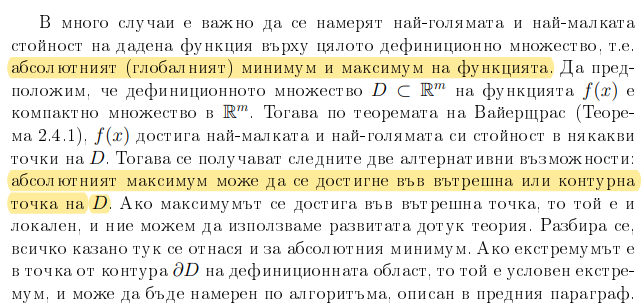
\includegraphics{Pics/calc/lec8-1.png}
  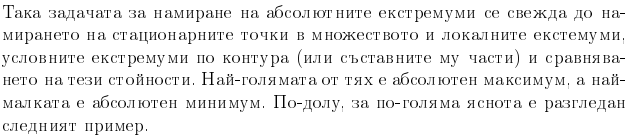
\includegraphics{Pics/calc/lec8-2.png}
\end{figure}

\begin{example}
Ако $E \subset \mathbb{R}^2, (x,y) \in \mathbb{R}^2, x \geq -1, y \geq -1, x+y \leq 1$ да се намерят най малката и най голямата стойност на функцията $f(x,y) = x^2 + y^2$ върху Е.\\
Решение:
\begin{gather*}
M_0 = (0,0) \in E \\
\Delta = 2 \cdot 2 - 0^2 >0 \quad f''_{xx} = 2 > 0 \implies f_{min} \\
f_{min} = f(0,0) = 0 \\
L(x,y;\lambda) = f(x,y) + \lambda(x+y-1) = x^2 + y^2 + \lambda(x+y-1) \\
L'_x = 2x + \lambda \quad L'_y = 2y + \lambda \\
\begin{array}{|l@{}}
2x + \lambda = 0\\
2y + \lambda = 0
x+y - 1 = 0
\end{array} \Leftrightarrow 
\begin{array}{|l@{}}
x = - \frac{\lambda}{2} \\
y= - \frac{\lambda}{2} \\
\lambda  = -1
\end{array} 
\implies M_1 \left( \frac{1}{2},\frac{1}{2} \right) 
\end{gather*}

\begin{gather*}
L''_{xx} = 2 \quad L''_{yy} = 2 \quad L''_{xy} = L''_{yx} = 0 \\
f_{min} = f(M_1)  = \frac{1}{4} + \frac{1}{4} = \frac{1}{2}\\
x = -1 \Leftrightarrow g(y) = (-1)^2 + y^2 = y^2 + 1 \\
g_{min} = g(0) = 1 = f_{min} \implies M_2(-1,0)\\
y = -1 \Leftrightarrow h(x) = x^2 + (-1)^2 = x^2 + 1 \\
h_{min} = h(0) = 1 = f_{min} \implies M_3(0,-1) \quad f(M_3) = 1\\
\begin{array}{|l@{}}
x + y = 1 \\
y = -1\\
\end{array}  \implies M_4(2,-1) 
\qquad 
\begin{array}{|l@{}}
x + y = 1  \\
x = -1\\
\end{array}  \implies M_5(-1,2) \\
f(-1,-1) = 2  \quad f(2,-1) = 5 \quad f(-1,2) = 5
\end{gather*}

\end{example}

\newpage
\section{Лекция 9}







\end{document}